\chapter{对偶}



    \section{内容引入}
        \paragraph{}任何一个线性规划或者写一个线性规划其实你得到的不是一个东西,而是两个东西,这另外一个东西就是他的对偶。 
    \section{对偶的用处}
        \paragraph{}我们之所以要讲对偶,对偶的作用如下:
        \begin{enumerate}
        \item 第一点用处是再往后了,等到我们讲近似算法的时候,非常重要,我们经常碰到一些优化一个目标函数,比如说最小化$f(\bm{x})$,但是最小化$f(\bm{x})$,有时候可能是NP完全的,是非常难的,所以我们只好求近似,不求最优求个差不多,求近似的时候如果我们一开始就知道$f(\bm{x})$的界,就非常有帮助,那怎么得到这种界呢,这种界还有一个用处就是在分支限界里面,千方百计得到一个界,对偶和松弛是非常有力的一种形式的界,所以我们要将对偶。
        \item 第二点用处是线性规划一般是成对出现的,我们写了一个LP之后,马上就可以写出对偶形式出来,所以我们就得到两个。那写了这个对偶之后怎么得到这个界呢?同时得到两个问题,对于其中一个问题的可行解就天然的是另外一个问题的一个界。
        \end{enumerate}
       
    \section{DIET问题}
    
    \subsection{原始问题}
    	\paragraph{}我们还是先从上面这最简单的例子看起,从家庭主妇买食品的例子入手,我们先回顾一下家庭主妇买食品,家庭主妇呢在市场上有这四种食品,每种食品他的成分都清楚,价格也知道,家庭主妇呢又想知道这一天呢我每种食品各买多少,使我花的钱最少,同时满足我能量的基本需求,我们已经讲过了,碰见这种问题我们怎么构建动态规划,这里面WILL?对象联系起来,还得稍微重塑一下。
        \paragraph{问题:}家庭主妇想知道她每天必须花费在食品上多少钱,以获得所有的能量(2000大卡),蛋白质(55克),钙(800毫克)。
        \paragraph{表格:}
        \ \\
        		\begin{table}[h]
        			\centering
					\begin{tabular}{l|ccc|c|c}			
					\hline
      		 			Food & Energy & Protein & Calcium  & Price & \textcolor{red}{Quantity}\\
 					\hline
 						Oatmeal & 110 & 4 & 2 & 3 & \textcolor{red}{$x_1$}\\
 						Whole milk & 160 & 8 & 285 & 9 & \textcolor{red}{$x_2$}\\
 						Cherry pie & 420 & 4 & 22 & 20 & \textcolor{red}{$x_3$}\\
 						Pork beans & 260 & 14 & 80 & 19 & \textcolor{red}{$x_4$}\\
					\hline
     				\end{tabular}
		 		\end{table}
        	
        \paragraph{线性规划方程:}
        \[
			\begin{array}{rrrrrrrrlr}
			 \min & 3x_1   &+& 9 x_2   &+& 20x_3   &+& 19x_4   & & \text{money}\\
 			s.t. & 110x_1 &+& 160 x_2 &+& 420 x_3 &+& 260 x_4 & \geq 2000 & \text{energy} \\
     		 & 4 x_1  &+& 8 x_2   &+& 4 x_3   &+& 14 x_4  & \geq 55 & \text{protein}\\
     			 &  2 x_1 &+& 285 x_2 &+& 22 x_3  &+& 80 x_4  & \geq 800 & \text{calcium}\\
     		 & x_1    &,& x_2     &,& x_3     &,&    x_4  & \geq 0 \\ 		
			\end{array} \nonumber
		\] 
		
		\paragraph{}我们的目标函数是什么呢?目标函数就是$3x_1+9x_2 + 20x_3   +19x_4$这是我们的总价格,我们总共要花多少钱,约束是什么呢?我们只看一个吧,能量约束,买$x_1$份燕麦我们要得到这么多能量,所以得到能量为$110x_1 + 160 x_2 + 420 x_3 + 260 x_4$,最小需求呢是2000大卡,所以约束是这个意思。
		
        
    \subsection{对偶问题}
    	\paragraph{}这个市场上总是有两类商品,不是只有一类,不仅有卖原始的燕麦、牛奶这些商品,还有一些公司呢分解的成果,比如说他是卖蛋白粉,单卖蛋白粉,单卖能量棒,单卖钙片。
    	\paragraph{问题表格:}
            \ \\     		
    		\begin{table}[h]   
    			\centering
    			\begin{tabular}{l|ccc|c}\hline
       				Food & Energy & Protein & Calcium  & Price (cents) \\
 					\hline
 					Oatmeal & 110 & 4 & 2 & 3 \\
					Whole milk & 160 & 8 & 285 & 9 \\
 					Cherry pie & 420 & 4 & 22 & 20 \\
 					Pork with beans & 260 & 14 & 80 & 19 \\    \hline
					\textcolor{blue}{ Price} & \textcolor{blue}{$y_1$} & \textcolor{blue}{$y_2$} & \textcolor{blue}{$y_3$} &   \\
					\hline
     			\end{tabular}
 			\end{table}
    	\paragraph{线性规划方程:}
    		\[
			\begin{array}{rrrrrrrrl}
 			\max & 2000 y_1   &+& 55 y_2   &+& 800 y_3 & &  &\text{money}   \\
			 s.t. & 110 y_1 &+& 4 y_2 &+& 2 y_3   & \leq &3 & \text{oatmeal} \\
  		     & 160 y_1 &+& 8 y_2 &+& 285 y_3 & \leq &9 & \text{milk} \\
   		     & 420 y_1 &+& 4 y_2 &+& 22 y_3  & \leq &20 & \text{pie} \\
             & 260 y_1 &+& 14 y_2 &+& 80 y_3  & \leq &19 & \text{pork\&beans} \\
             &     y_1 &,&    y_2 &,&    y_3  &  \geq & 0 \\ 		
			\end{array} \nonumber
			\]
		\paragraph{}那假如说你是卖蛋白粉的商家,如果让你来定价格,你应该怎么来定?首先说这个价格,你的总体目标当然是想赚的钱越多越好,每个家庭主妇都要赚的越多钱越好,另外当然你这个价格有一些限制条件,如果你定的价格与原始商品的价格之间有竞争力,家庭主妇就可能考虑购买你的商品,比如不吃燕麦了买一堆的蛋白粉,一堆的能量棒和钙片,混在一块效果和麦片一样。但是你价格定的过高呢,那家庭主妇还不如直接去买麦片,这是一个很简单的道理。
		\paragraph{}接着我们会考虑到如果你是这个商家,让你来定一个合理的价格,你怎么定呢?你只好写一个这样的线性规划,我们假设能量棒是$y_1$,1大卡的能量棒我们的定价是$y_1$,1克的蛋白我们定价$y_2$,1毫克的钙是$y_3$,$2000 y_1 + 55 y_2 + 800 y_3$就是我在一个家庭主妇身上至少赚这么多钱,我的目标就是至少赚的钱,最大化它。下面第一个约束是说各种成分的价格总和一定小于燕麦的价格,不然家庭主妇就会直接购买燕麦。那这个商家要定这个价格,并且在市场上价格越高越好,那么他就必须解这个线性规划。
		\subsection{DIET问题总结}
		\paragraph{}从DIET这个例子中我们可以看出,假如将原先的家庭主妇的问题定为原问题,那这个商家定价的问题就定为对偶问题,这两个是非常紧密关联的,实际上原问题和对偶问题只不过是矩阵$\bm{A}$的两种看法:家庭主妇是按照行看,商家问题是按照列看。家庭主妇问题按行看写成矩阵的样子就是:min $\bm{c^Tx}$。商家问题按列看携程矩阵的样子就是:max $\bm{y^Tb}$。基本上两个式子是完全对应的。
		
		\section{原始问题和对偶问题}
		\subsection{线性规划矩阵}
			\[
			\begin{array}{rrrrrrrrrrrrl}
     			& c_1    & &  c_2    & &  ...& & c_n     &      &    & \\
      			&   & & & & & & & & & \\
      			& a_{11}  & & a_{12}  & & ... & & a_{1n} &   & b_1 &  \\
           		&   & & & & & & & & & \\
      			& a_{21} & & a_{22}  & & ... & & a_{2n}  &   & b_2 &  \\
             	&   & & & & & & & & & \\
      			&           & &           & & ... & &           &      &     &  \\
             	&   & & & & & & & & & \\
      			& a_{m1} & & a_{m2}  & & ... & & a_{mn}  &  & b_m &  \\
         	\end{array} \nonumber
			\]
			
			\paragraph{}原始问题和对偶问题只是对于线性规划矩阵A两种不同的角度:
			\begin{itemize}
				\item 原始问题:从行看
				\item 对偶问题:从列看
			\end{itemize}
		\subsection{原始问题}
			\paragraph{详细表示(按行看):}
			\[
			\begin{array}{rrrrrrrrrrrrl}
				\textcolor{red}{ \min} & c_1\textcolor{red}{ x_1}    &+&  c_2\textcolor{red}{ x_2}   &+&  ...&+& c_n\textcolor{red}{ x_n}    &      &    & \\
       			&   & & & & & & & & & \\
      			& a_{11}\textcolor{red}{ x_1} &+& a_{12}\textcolor{red}{ x_2} &+& ... &+& a_{1n}\textcolor{red}{ x_n }& \textcolor{red}{\geq} & b_1 &  \\
           		&   & & & & & & & & & \\
      			& a_{21}\textcolor{red}{ x_1} &+& a_{22}\textcolor{red}{ x_2} &+& ... &+& a_{2n}\textcolor{red}{ x_n} & \textcolor{red}{\geq} & b_2 &  \\
             	&   & & & & & & & & & \\
      			&           & &           & & ... & &           &      &     &  \\
             	&   & & & & & & & & & \\
     			& a_{m1}\textcolor{red}{ x_1} &+& a_{m2}\textcolor{red}{ x_2} &+& ... &+& a_{mn}\textcolor{red}{ x_n} & \textcolor{red}{\geq} & b_m &  \\
      			&           & &           & &     & &       x_i & \geq & 0   & \text{for each }  i \\
     		\end{array} \nonumber
			\]
			\paragraph{矩阵表示:}
			\[
			\begin{array}{rrrrrrrrl}
 				\min & \mathbf{ c^T x} &    \\
 				s.t. & \mathbf{A x} &  \mathbf{\geq b}   \\
      			&\mathbf{x} &  \mathbf{\geq 0 }\\
				\end{array} \nonumber
			\]
		\subsection{对偶问题}
			\paragraph{详细表示(按列看):}
				\[
				\begin{array}{cccccccccrrrrl}
   					c_1     &   &  c_2    & &  ...& & c_n     &      &    & \\
  					\reflectbox{\rotatebox[origin=c]{270}{\textcolor{blue}{$\geq$} }}    &   &    \reflectbox{\rotatebox[origin=c]{270}{\textcolor{blue}{$\geq$} }}    & &     & &  \reflectbox{\rotatebox[origin=c]{270}{\textcolor{blue}{$\geq$} }}     &      &   \textcolor{blue}{\max } &     \\                                           
   					\textcolor{blue}{y_{1}} a_{11}  &   & \textcolor{blue}{y_{1}}a_{12}  &  & ... &  & \textcolor{blue}{y_{1}}a_{1n}  &                                & \textcolor{blue}{y_{1}}b_1 &  \\
     				+            &   &  +              &  &     &   & +              &                                 & +  & \\
    				\textcolor{blue}{y_{2}}a_{21}   &  & \textcolor{blue}{y_{2}}a_{22}  &  & ... &  & \textcolor{blue}{y_{2}}a_{2n}  &                             & \textcolor{blue}{y_{2}}b_2  &  \\
     				 +            &   &  +              &  &     &   & +              &                                 & +  & \\
        			\vdots      & &   \vdots          & & ... & &    \vdots         &      &   \vdots    &  \\
      				+            &   &  +              &  &     &   & +              &                                 & +  & \\
    				\textcolor{blue}{y_{m}}a_{m1} &  &  \textcolor{blue}{y_{m}}a_{m2}  &  & ... &  & \textcolor{blue}{ y_{m}}a_{mn}  &                          & \textcolor{blue}{y_{m}}b_m &  \\
              		& &           & &     & &       y_j & \geq & 0   & \text{for each }  j \\
				\end{array} \nonumber
				\]
			\paragraph{矩阵表示:}
				\[
				\begin{array}{rrl}
 					\max & \mathbf{y^T b} &      \\
 					s.t. & \mathbf{y}   & \mathbf{\geq 0 } \\
      				& \mathbf{y^T A} &  \mathbf{\leq  c^{T} }   \\
				\end{array} \nonumber
				\]
				
			\subsection{原始问题与对偶问题之间的转换}
			\paragraph{}写出一个线性规划的时候,可以同时得到他的对偶。原问题为Min时,那么对偶就是Max:
				\begin{itemize}
					\item 一旦原问题是$\bm{Ax} \leq \bm{b}$,那么对偶一定是$\bm{y} \leq 0$;一旦原问题是$\bm{x} \geq 0$,那么对偶问题就是$\bm{y^TA \leq c}$。
						\begin{figure}[h]
							\centering
 							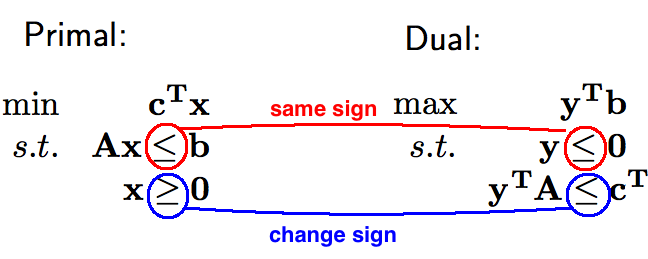
\includegraphics[width=2.5in] {L9-primaldual-case1.png}
						\end{figure}
						
					\item 如果原始问题是$\bm{Ax} = b$,那么对偶问题对$\bm{y}$没有约束,你可以$\bm{y} \leq 0 $也可以$\bm{y} \geq 0$;$\bm{x} \geq 0$一样需要反号。
						\begin{figure}[h]
							\centering
 							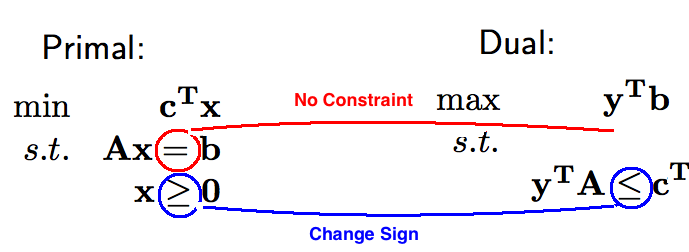
\includegraphics[width=2.5in] {L9-primaldual-case2.png}
						\end{figure}
					
				\end{itemize}				
							
		\section{拉格朗日乘子和KKT条件}
			\paragraph{}我们写出一个线性规划,那么我们就可以机械的写出他的对偶。对偶为何要这样生成,我们可以很容易的从拉格朗日对偶的观点中得出。
		\subsection{拉格朗日乘子}
		\subsubsection{引入}
			\paragraph{}拉格朗日是:求min $f(\bm{x})$,我们可以通过倒数等于零,如果给我们约束min $f(\bm{x})$,一定要满足等式$g_i(\bm{x}) = 0$ 的条件,再增加难度,再加入不等式条件$h_i(\bm{x}) \leq 0$。
			\paragraph{}即以下三步:
			\begin{enumerate}
				\item 首先没有约束条件。
					 \[
  					     \min\ f( \mathbf{x} )
  					 \] 
				\item 加入等式条件$g_i(\bm{x}) = 0$。
					\[
					\begin{array}{rrrrrrrrl}
 						\min & f( \mathbf{x})  &  & & \\
 						s.t. & g_i( \mathbf{x}) & \textcolor{red}{\bf =} &0 & i=1,2,..., m \\
					\end{array} \nonumber
					\]
				\item 再加入不等式条件$h_i(\bm{x}) \leq 0$。
					\[
					\begin{array}{rrrrrrrrl}
 						\min & f( \mathbf{x})  &  & & \\
 						s.t. & g_i( \mathbf{x}) & \textcolor{red}{\bf =} &0  & i=1,2,..., m \\
       					& h_i( \mathbf{x}) & \textcolor{red}{\bf \leq} &0  & i=1,2,..., p 
					\end{array} \nonumber
					\]
			\end{enumerate}
		\subsubsection{求解}
			\paragraph{}我们考虑以下问题:
				\[
				\begin{array}{rrrrrrrrl}
 					\min & f(x,y)  &   &\\
 					s.t. & g(x,y)  & \textcolor{red}{\bf =} & 0
				\end{array} \nonumber
				\]
			\paragraph{}我们把$g(x,y) = 0$这条曲线画在图上,把$f(x,y)$画等高线,比如说图上等于1和2,我们的目标是要在$g(x,y) = 0$这条曲线上找一个点使得$f(x,y)$越小越好。
			
			\begin{figure}[h]
			\centering
				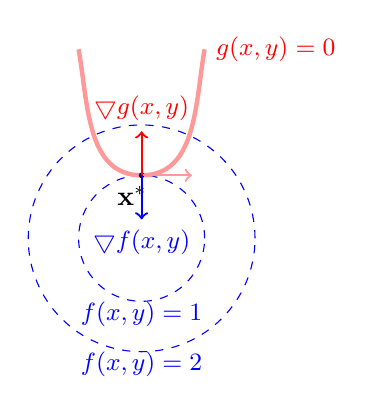
\begin{tikzpicture}[scale=0.8, auto,swap]
 
 				%\draw[<->,  thick] (0,4) node[thick, left]{$y$}-- (0,0) -- (4,0) node[ultra thick, below] {$x$};
				\draw[dashed, blue] (1,1) circle[radius=1.8]; 
				\draw[dashed, blue] (1,1) circle[radius=1];
				%\draw[dashed, blue] (1,1) circle[radius=0.5];
				%\draw[fill=blue] (1,1) circle[radius=1pt];

				\draw[ultra thick, red!40] (0,4) to[out=280, in=180] (1,2) to[out=0, in=260] (2,4) node[red, right]{\small $g(x, y)=0$};

				\draw[fill=blue] (1,2) circle[radius=1pt];

				\node[black, ultra thick, below ] at (0.85,2) {$\mathbf{x}^{*}$}; 
				\draw[->,  thick, red!40] (1,2) -- (1.8, 2);
				\draw[->,  thick, red] (1,2) -- (1, 2.7) node[above]{\small $\bigtriangledown g(x, y)$};
				\draw[->, thick, blue] (1,2) -- (1, 1.3) node[below]{\small $\bigtriangledown f(x, y)$}; 
 
				\node[blue, ultra thick ] at (1,-0.2) {\small  $f(x,y)=1$}; 
				\node[blue, ultra thick] at (1,-1) {\small  $f(x,y)=2$}; 
        
			\end{tikzpicture}
			\end{figure}
			\paragraph{}我们就把它想成气球,这个气球一开始比较大,这上面与$g(x,y) = 0$交了两个点,这时候能找到两个点且$f(x,y)$等于2,然后我们尝试$f(x,y)$变小,直到与$g(x,y) = 0$有一个交点,最后变成没有交点,这个时候$f(x,y)$达到最小,所以可以得到最后最小的点肯定是$g(x,y)$与等高线若近若离的,这个若近若离的表示方法就是$g(x,y) = 0$与等高线相切的,那个点就是最优点。
			\paragraph{}所以得到以下式子:
			\begin{itemize}
				\item  
						$\bigtriangledown f(x, y) = \lambda \bigtriangledown g(x, y)$
				\item  
						$L(x,y,\lambda) = f(x,y) - \lambda g(x,y) $
				\item
						$\bigtriangledown L(x^*, y^*, \lambda) = 0$
			\end{itemize}
			\paragraph{}我们将相切继续表示,表示成它们的法线,也就是梯度,这个梯度都会垂直于这个切线,所以我们直观上看,假如说$(x^*,y^*)$是最优解的话,那么在这个点上$f(x,y)$不会再改变值了,沿着这条线走的话$f(x,y)$数值不变,也就是说他两的梯度要在同一条直线上,有可能同向也有可能反向。可以表示为两个梯度成一定比例,我们把比例用$\lambda$表示$\bigtriangledown f(x, y) = \lambda \bigtriangledown g(x, y)$,接着就可以得到拉格朗日方程$L(x,y,\lambda) = f(x,y) - \lambda g(x,y) $,接着对于拉格朗日方程求导,等于0可以得到$\bigtriangledown f(x, y) = \lambda \bigtriangledown g(x, y)$,所以得到求有约束的最小值,可以转化成$\bigtriangledown L(x^*, y^*, \lambda) = 0$。
			\paragraph{}朗格朗日方程式原始的优化目标减去一个东西,这个东西可以看作是违反约束的阀,因为我们要求约束的结果等于0,如果$g(x,y)$不等于0那么我们就要减去后面这个式子,这个$\lambda$就是拉格朗日乘子。
			\paragraph{拉格朗日乘子:}
			\begin{center}
				$L(x,y,\lambda) = f(x,y) - \lambda g(x,y) $
			\end{center}
		\subsection{KKT条件}
		\paragraph{}前面我们已经完成了约束为$g(x) = 0$的求解方法,那如果是小于等于0,那就不在是拉格朗日了,是拉格朗日的拓展,叫KKT条件。
		\subsubsection{引入}
		\paragraph{}要求$g(x,y) \leq 0$,也就是说图中的阴影区我们是要在阴影区或者边界上找一个点,使得$f(x,y)$最小,我们把他分成两种情况:
		\begin{enumerate}
			\item 如果最优解恰好在这条边界上,那么这个就可以通过拉格朗日来求解。
			\item 如果最优解在阴影区内部,我们是要找最优解,这个最优解不在边界上,在他内部,如果在内部那这个解一定是单纯考虑$f(x,y)$的最优解,也就是直接求$\bigtriangledown f(x,y) = 0$的解。
		\end{enumerate}
		\begin{figure}[h]
		\centering
\begin{minipage}{0.49\textwidth}
\centering
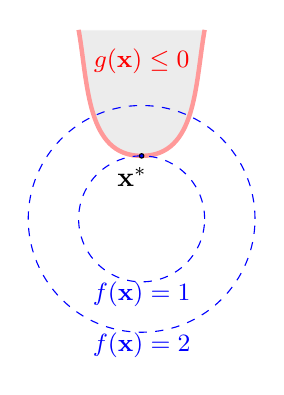
\begin{tikzpicture}[scale=0.8, auto,swap]
 
 %\draw[<->,  thick] (0,4) node[thick, left]{$y$}-- (0,0) -- (4,0) node[ultra thick, below] {$x$};
\draw[white, fill=gray!15] (0,4) to[out=280, in=180] (1,2) to[out=0, in=260] (2,4) -- (0,4);
\draw[ultra thick, red!40] (0,4) to[out=280, in=180] (1,2) to[out=0, in=260] (2,4); 
\node[ultra thick, red] at (1,3.5) {\small $g(\mathbf{x})\leq 0$}; 

\draw[dashed, blue] (1,1) circle[radius=1.8]; 
\draw[dashed, blue] (1,1) circle[radius=1];

%\draw[fill=blue] (1,1) circle[radius=1pt];


\draw[fill=blue] (1,2) circle[radius=1pt];

 \node[black, ultra thick, below ] at (0.85,2) {$\mathbf{x}^{*}$}; 
%\draw[->,  thick, red!40] (1,2) -- (1.8, 2);
%\draw[->,  thick, red] (1,2) -- (1, 2.7) node[above]{\small $\bigtriangledown g(x, y)$};
 %\draw[->, thick, blue] (1,2) -- (1, 1.3) node[below]{\small $\bigtriangledown f(x, y)$}; 
 
  \node[blue, ultra thick ] at (1,-0.2) {\small  $f(\mathbf{x})=1$}; 
 \node[blue, ultra thick] at (1,-1) {\small  $f(\mathbf{x})=2$}; 

        
\end{tikzpicture}
\end{minipage}
\begin{minipage}{0.49\textwidth}
\centering
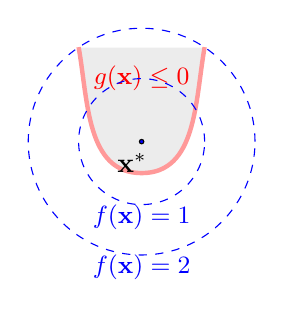
\begin{tikzpicture}[scale=0.8, auto,swap]
 
 %\draw[<->,  thick] (0,4) node[thick, left]{$y$}-- (0,0) -- (4,0) node[ultra thick, below] {$x$};
\draw[white, fill=gray!15] (0,4-1.5) to[out=280, in=180] (1,2-1.5) to[out=0, in=260] (2,4-1.5) -- (0,4-1.5);
\draw[ultra thick, red!40] (0,4-1.5) to[out=280, in=180] (1,2-1.5) to[out=0, in=260] (2,4-1.5); 
\node[ultra thick, red] at (1,3.5-1.5) {\small $g(\mathbf{x})\leq 0$}; 

\draw[dashed, blue] (1,1) circle[radius=1.8]; 
\draw[dashed, blue] (1,1) circle[radius=1];

\draw[fill=blue] (1,1) circle[radius=1pt];


%\draw[fill=blue] (1,2) circle[radius=1pt];

 \node[black, ultra thick, below ] at (0.85,1) {$\mathbf{x}^{*}$}; 
%\draw[->,  thick, red!40] (1,2) -- (1.8, 2);
%\draw[->,  thick, red] (1,2) -- (1, 2.7) node[above]{\small $\bigtriangledown g(x, y)$};
 %\draw[->, thick, blue] (1,2) -- (1, 1.3) node[below]{\small $\bigtriangledown f(x, y)$}; 
 
  \node[blue, ultra thick ] at (1,-0.2) {\small  $f(\mathbf{x})=1$}; 
 \node[blue, ultra thick] at (1,-1) {\small  $f(\mathbf{x})=2$}; 

        
\end{tikzpicture}
\end{minipage}
\end{figure}
		\subsubsection{满足条件}
		\paragraph{}KKT条件可以这样来表示,首先先写一个拉格朗日$L(x,y,\lambda) = f(x,y) - \lambda g(x,y) $,这个最优解需要满足的条件就是:
		\begin{enumerate}
			\item 与拉格朗日一样,使得式子的倒数等于0。
			\item 满足原先的可行性,原先的$g(x,y) \leq 0$。
			\item 对偶的可行性$ \lambda_i \leq 0 $。
			\item 满足互补的松弛性。每个$ \lambda_ig_i(x) = 0$。
		\end{enumerate}
	\section{向线性规划中引入拉格朗日对偶}
	\subsection{拉格朗日对偶}
	\paragraph{}对于线性规划:
		\[
		\begin{array}{rrrrrrrrl}
 			\min & \mathbf{c^T x} &  & \\
 			s.t. & \mathbf{A x } & \geq&  \mathbf{b }\\
      		& \mathbf{x} & \geq& \mathbf{0} 
		\end{array} \nonumber
		\]
	\paragraph{}这是一个约束优化问题,反正对于约束优化问题都可以写出拉格朗日,拉格朗日是对每一个约束加了一个$\lambda$,变成:
	\[
		L(\mathbf{x, \lambda}) = \mathbf{c^Tx} - \sum\nolimits_{i=1}^m \lambda_i ( a_{i1}x_{1} + a_{i2}x_{2} + ... a_{in}x_{n}  - b_i) 
	\]
	\paragraph{}如果我们要求$\lambda \geq 0$,并且$\bm{x}$是可行解的话,那么我们原先的目标函数肯定比$L(\bm{x},\lambda)$要大。
	\paragraph{}对于$g(\mathbf{\lambda} ) = \inf_{\mathbf{x} } L( \mathbf{x}, \mathbf{\lambda} )$,就是对于任意的$\lambda$我都把所有的$\bm{x}$都枚举一遍,算出它的下界当中最大的下区界,所以$L(\bm{x},\lambda)$一定大于等于$g(\lambda)$。这里的$g(\lambda)$就是拉格朗日对偶。
	\paragraph{}现在对于拉格朗日对偶进行解释,得到以下求解过程:
	\begin{eqnarray}
 		g(\mathbf{\lambda}) &= & \inf_{\mathbf{x}} L( \mathbf{x, \lambda} ) \nonumber \\
            				&=& \inf_{\mathbf{x}} ( \mathbf{c^Tx} - \sum\nolimits_{i=1}^m \lambda_i ( a_{i1}x_{1} + a_{i2}x_{2} + ... a_{in}x_{n}  - b_i) ) \nonumber \\
            				&=& \inf_{\mathbf{x}} (\mathbf{c^Tx - \lambda^T(Ax-b)})  \nonumber \\
            				&=& \inf_{\mathbf{x}} ( \mathbf{c^Tx - \lambda^TAx+\lambda^Tb}) \nonumber\\
            				&=& \inf_{\mathbf{x} } (  \mathbf{ \lambda^T b + (c^T - \lambda^T A) x } ) \nonumber\\
            				&=& \begin{cases} 
                        			\mathbf{ \lambda^T b}  & \text{if } \mathbf{ c^T \geq \lambda^T A} \text{\ and \ }  \mathbf{x \geq 0} \\ 
                         			-\infty         & \text{otherwise}
                     			\end{cases} \nonumber
	\end{eqnarray}
	\subsection{强边界}
	\paragraph{}现在我们给出任意一个$f(\bm{x})$,我们现在可以通过拉格朗日搭一下桥,我们想min $f(\bm{x})$,现在可以得到$f(\bm{x}) \geq L(\bm{x},\lambda) \geq g(\lambda)$,所以得到我要min $f(\bm{x})$,最小最小不可能比$g(\lambda)$要小了,所以我们就max $g(\lambda)$,任何一个$g(\lambda)$都要比$f(\bm{x})$要小,所以最大的值就是$f(\bm{x})$的最小值,所以将$\lambda$换成$\bm{y}$就是我们所要得到的对偶。
	\subsection{例子}
	\paragraph{}接着看一个例子,原问题是:
		\[
		\begin{array}{rrrrrrrrl}
 			\min & x & &   \\
 			s.t. & x & \geq& 2 \\ 
      			 & x & \geq& 0 
		\end{array} \nonumber
		\]
	\paragraph{}写出他的拉格朗日为:
	\begin{center}
		$L(x,y) = x - y*(x-2 ) = 2y + x*(1-y)$ 
	\end{center}
	\paragraph{}所以拉格朗日对偶为:
	\begin{center}
		$g(y) = \inf_x L(x,y) =  \begin{cases} 2 y & \text{ if } x\geq 0 \text{ and } (1-y)\geq 0  \\ 
                                                          -\infty & \text{ otherwise } 
                                     \end{cases} $
	\end{center}
	\paragraph{}所以对偶问题为:
	\[
	\begin{array}{rrrrrrrrl}
 		\max & 2y    \\
 		s.t. & y  \leq 1 \\ 
      		 & y  \geq 0 
	\end{array} \nonumber
	\]
	\subsection{拉格朗日——原问题和对偶问题之间的桥梁}
		\paragraph{}核心的问题是,我们原先要min的目标函数大于等于拉格朗日,拉格朗日大于等于对偶目标函数,也就是说min $\mathbf{c^Tx} \geq \mathbf{L(x,y)} \geq \mathbf{y^Tb}$,所以通过拉格朗日搭了一下桥,所以我们原先的目标函数一定大于对偶的目标函数。图下图所示:
		\begin{figure}[h]
			\centering
 			\includegraphics[width=2.4in,angle=-90] {L9-Lagrangian-dual.eps}
		\end{figure}
     \subsection{对偶变量$\bm{y}$}
     \paragraph{}对偶用途非常广,尤其在经济学领域,经常把它叫做一个价格,经济学领域中常常用到线性规划,常常把对偶变量$\bm{y}$叫做影子价格或者叫边界成本。边界成本就是说,当我们放松或者加强一个东西的时候,你要多少钱。边界成本就是拉格朗日乘子。
     \paragraph{}拉格朗日乘子就是说我违反了任意一个约束的时候你要罚我多少钱,我们原本的约束是$\bm{Ax} \geq b$,违反了以后就变成了$b_i + \Delta b_i$,变了一点点,那要罚我都少钱呢?那罚的钱数目就是$\frac{\partial L(\mathbf{x}, \mathbf{\lambda})}{\partial b_{i}} = \lambda_{i}$。
     \paragraph{}通过例子可以看出对偶变量就是拉格朗日乘子。拉格朗日乘子就是约束稍微改变一点,对于目标函数有什么变化,有的改变对于目标函数没有变化,有的有变化,这个变化多少就是拉格朗日乘子就是我们的对偶变量。
     \paragraph{例子:} \ \\
     \paragraph{}DIET问题的$\bm{b}$的值为$b_1=2000, b_2 = 55, b_3=800$,原始问题的可行解:\\
     	\begin{align*}
		 	    \mathbf{x}&=(14.24, 2.70, 0, 0) \\
		        \mathbf{c^Tx}&=67.096
     	\end{align*}
     \paragraph{}对偶问题的可行解:
     	\begin{align*}
     		\mathbf{y}&=(0.0269, 0, 0.0164) \\
			\mathbf{y^Tb}&=67.096  
     	\end{align*}
     \paragraph{}稍稍改变$\bm{b}$,看对于max $\mathbf{c^Tx}$的影响:
     	\begin{itemize}
     		\item $b_1= 2001$: $\max \mathbf{c^Tx}=67.123$ \ \ ($\mathbf{y_1}=0.0269 = 67.123 - 67.096$)
			\item $b_2=\quad 56$: $\max \mathbf{c^Tx}=67.096$ \ ($\mathbf{y_2}=0  = 67.096 - 67.096$)
			\item $b_3=\ \ 801$: $\max \mathbf{c^Tx}=67.112$ ($\mathbf{y_3}=0.0164  = 67.112 - 67.096$)
     	\end{itemize}
     \section{对偶的四个性质}
     \subsection{性质一:对偶的对偶就是原问题}
     \paragraph{}原始问题(P):
     	\[
		\begin{array}{rrrrrrrrl}
 			\min & \mathbf{c^T x} &  & \\
 			s.t. & \mathbf{A x } & \geq&  \mathbf{b }\\
      		& \mathbf{x} & \geq& \mathbf{0} 
		\end{array} \nonumber
		\]
     \paragraph{}对偶问题(D):
     	\[
		\begin{array}{rrrrrrrrl}
 			\max & \mathbf{y^T b} &  & \\
 			s.t. & \mathbf{x} & \geq& \mathbf{0} \\
 				 & \mathbf{y^T A } & \leq&  \mathbf{c^T }
		\end{array} \nonumber
		\]
     \paragraph{}对偶的改变($D'$):
     	\[
		\begin{array}{rrrrrrrrl}
 			\min & \mathbf{y^T (-b)} &  & \\
 			s.t. & \mathbf{x} & \geq& \mathbf{0} \\
 				 & \mathbf{y^T (-A) } & \geq&  \mathbf{(-c^T) }
		\end{array} \nonumber
		\]
     \paragraph{}对偶的对偶($D'D$):
     	\[
		\begin{array}{rrrrrrrrl}
 			\max & \mathbf{x^T (-c^T)} &  & \\
 			s.t. & \mathbf{x} & \geq& \mathbf{0} \\
 				 & \mathbf{x^T (-A) } & \leq&  \mathbf{-b^T }
		\end{array} \nonumber
		\]
		\begin{center}
			与原问题相同
		\end{center}
	\subsection{性质二:弱对偶性}
		\subsubsection{内容}
		\paragraph{}\textbf{对于一般问题,对偶问题的任意一个可行解总是原问题的一个下界。}
		\subsubsection{例子}
		\begin{figure}[h]
			\centering
 			\includegraphics[width=2.4in,angle=-90] {L9-Lagrangian-dual.eps}
		\end{figure}
		\subsubsection{证明}
		\paragraph{原始问题:}
			\[
			\begin{array}{rrrrrrrrl}
				\min & \mathbf{c^T x}  &   \\
 				s.t.  & \mathbf{A x } & \mathbf{ \geq  b }  \\
 					  & \mathbf{x  } & \mathbf{ \geq 0 } 
 			\end{array} \nonumber
			\]
		\paragraph{对偶问题:}
			\[
			\begin{array}{rrl}
 				\max & \mathbf{y^T b} &    \\
 				s.t. & \mathbf{y}  & \mathbf{ \geq 0 }  \\
      				 	& \mathbf{y^T A} &  \mathbf{ \leq  c^{T} }  \\
			\end{array} \nonumber
			\]
		\paragraph{推导:}
		\begin{itemize}
			\item 由于$\mathbf{y^T A \leq c^T}$并且$\mathbf{x^T \geq 0}$,所以$\mathbf{c^T x \geq y^T A  x }$。
			\item 由于$\mathbf{Ax \geq b}$并且$\mathbf{y \geq 0}$,所以$\mathbf{c^T x \geq y^T A  x \geq y^T b }$。
		\end{itemize}
	\subsection{性质三:强对偶性}
	\subsubsection{内容}
	\paragraph{}\textbf{对于线性规划,原问题的存在最优解,那对偶问题也存在一个最优解,它们的数值相等。}
	\subsubsection{证明}
		\begin{itemize}
			\item 线性规划的最优解肯定能够写成$\mathbf{x^*= \left[ \begin{array}{c} \mathbf{B^{-1}b}\\ 0 \end{array}\right]}$,最优解肯定在顶点上,顶点就是一个基,假如这个基是$\mathbf{B}$则$\mathbf{x}$一定写成$\mathbf{B^{-1}b}$,其它的非基向量为0。且停止条件是$\mathbf{c^T - c_B^T B^{-1} A \geq 0}$。
			\item 我们定义:$\mathbf{y^{*T}={c_B}^T {B}^{-1}}$。$\mathbf{y^{*T}}$是对偶的最优解。
			\item 带入得到,$\mathbf{y^{*T} b = {c_B}^T {B}^{-1} b = {c}^T {x^*}}$。
			\item 因为所有的$\mathbf{y}$带入对偶问题都小于等于原始问题,现在找到一个相等的了,所以这个$\mathbf{y^*}$一定是最优解。
		\end{itemize}
	\subsection{性质四:互补松弛性}
	\subsubsection{内容}
	\paragraph{}\textbf{假如x是原问题的可行解,y为对偶问题的可行解,那么x和y是最优解时,当且仅当:}
		\begin{itemize}
			\item \textbf{对于任意$1\leq i \leq m$,$u_i =   y_i ( a_{i1}x_{1} + a_{i2}x_{2} + ... +a_{in}x_{n}  - b_i) = 0$。}
			\item \textbf{对于任意$1\leq j \leq n$,$v_j =  ( c_j - a_{1j}y_{1} - a_{2j}y_{2} - ... - a_{mj}y_{m} )x_j = 0$。}
		\end{itemize}
	\subsubsection{例子}
		{\sc Diet}问题的可行解和他的对偶问题的可行解是: $\mathbf{x}=(14.244, 2.707, 0, 0 )$ 和 $\mathbf{y}=(0.0269, 0, 0.0164)$。可以得到:
		\[
		\begin{array}{rrrrrrrrlr}
 			& 110x_1 &+& 160 x_2 &+& 420 x_3 &+& 260 x_4 & \textcolor{red}{=} 2000 & \\
      		& 4 x_1  &+& 8 x_2   &+& 4 x_3   &+& 14 x_4  & \textcolor{red}{>} 55 & \textcolor{red}{\Rightarrow y_2=0}\\
      		&  2 x_1 &+& 285 x_2 &+& 22 x_3  &+& 80 x_4  & \textcolor{red}{=} 800 & \\
      		& x_1    &,& x_2     &,& x_3     &,&    x_4  & \geq 0 \\ 		
		\end{array} \nonumber
		\] 
	\subsubsection{证明}
	\paragraph{证:}
		\begin{itemize}
		\item 对于任意$i$和$j$,$ u_i = 0 \text{ 并且 }  v_j = 0 $
		\item $ \Leftrightarrow \sum_i u_i = 0 \text{ 并且 } \sum_j v_j = 0 \text{ (因为 } u_i \geq 0, v_j \geq 0\text{)} $ 
		\item $ \Leftrightarrow  \sum_i u_i + \sum_j v_j = 0 $
		\item $\Leftrightarrow  \mathbf{ ( y^T A x - y^T b )+ ( c^T x - y^T A x ) = 0}  $
		\item $\Leftrightarrow  \mathbf{ y^T b = c^T x } $
		\item $\Leftrightarrow  \mathbf{y}  \text{ 和 } \mathbf{x}$  是可行解 (通过强对偶性质可以得到,$\mathbf{y^T b}$ 和 $\mathbf{c^T x}$ 到达了他们自身的边界)	
		\end{itemize}
	\section{原问题和对偶问题的9种情况}
	\paragraph{}给我们任何的实际问题,我们可以写出他的线性规划,然后我们就可以机械的写出他的对偶,然后分别进行求解。
	\begin{figure}[h]
		\centering
 		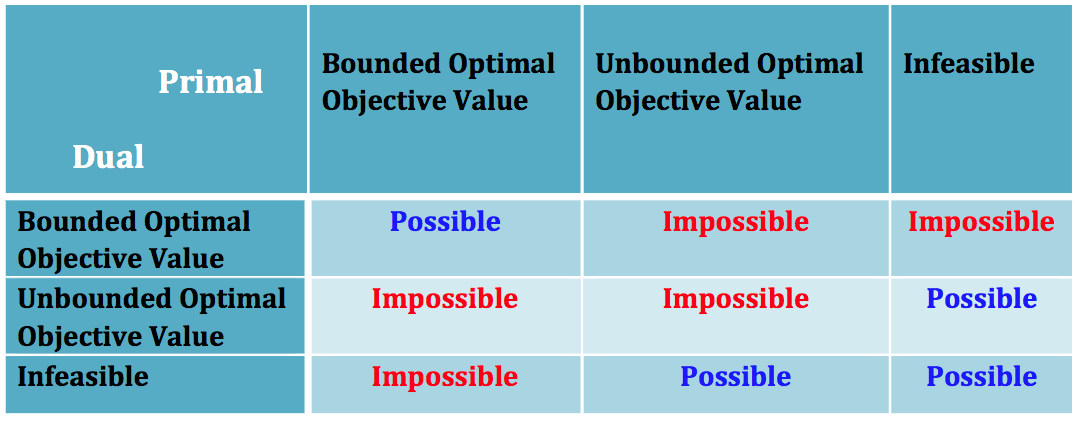
\includegraphics[width=4in] {L9-primaldual-table.png}
	\end{figure}
	\subsection{例子1:原问题有无界最优解,对偶问题无解}
	\begin{itemize}
		\item 原问题:
			\[
			\begin{array}{rrrrrrl}
 				\min & -2 x_1 & - & 2x_2 & \\
 				s.t. &   x_1 & - & x_2 & \leq & 1   \\
      			     & - x_1 & + & x_2 & \leq & 1   \\
      				 &   x_1 &   &         & \geq & 0   \\
            		 &      &  & x_2 & \geq & 0   
			\end{array} \nonumber
			\]
		\item 对偶问题
			\[
			\begin{array}{rrrrrrl}
 				\max & y_1 & + & y_2 & \\
 				s.t. &   y_1 & &         &       \leq & 0   \\
      				 &   &       &    y_2     & \leq & 0   \\
      				 &   y_1 & - & y_2  & \leq & -2   \\
      				 &   -y_1 &+ & y_2 & \leq & -2   \\
			\end{array} \nonumber
			\]
	\end{itemize}
	\subsection{例子2:原问题和对偶问题都无解}
		\begin{itemize}
			\item 原问题:
				\[
				\begin{array}{rrrrrrl}
 					\min &   x_1 & - & 2x_2 & \\
 					s.t. &   x_1 & - & x_2 & \geq & 2   \\
      					 & - x_1 & + & x_2 & \geq & -1   \\
      					 &   x_1 &   &         & \geq & 0   \\
            			 &      &  & x_2 & \geq & 0   
					\end{array} \nonumber
				\]
			\item 对偶问题:
				\[
				\begin{array}{rrrrrrl}
 					\max & 2y_1 & - & y_2 & \\
 					s.t. &   y_1 & &         &       \geq & 0   \\
      					 &   &       &    y_2     & \geq & 0   \\
     				     &   y_1 & - & y_2  & \leq & 1   \\
      					 &   -y_1 &+ & y_2 & \leq & -2   \\
				\end{array} \nonumber
				\]
		\end{itemize}
	\section{对偶应用1:Farkas引理}
		\subsection{引理内容}
			\paragraph{}给我一堆的向量$\mathbf{a_1, a_{2}, ..., a_{m}, c} \in \mathbb{R}^n$,那么就可以得到:
			\begin{enumerate}
				\item $\mathbf{c} \in \mathbf{C(a_{1}, a_{2},..., a_{m})}$,或者
				\item 存在一个向量$\mathbf{y}\in \mathbb{R}^{n}$,对于任意的$i$,$\mathbf{y^T a_i \geq 0}$ 但是 $\mathbf{ y^T c < 0}$ 成立。
			\end{enumerate}
		\subsection{引理图例解释}
		\begin{figure}[h]
\begin{minipage}{0.45\textwidth}
\centering
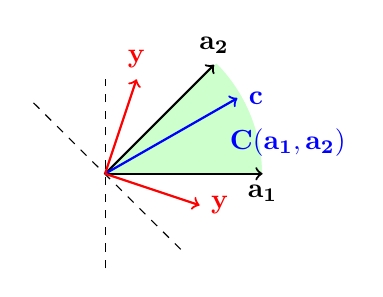
\begin{tikzpicture}[scale=0.8, auto,swap]
 
\draw[white, fill=green!20] (0,0) -- (2.5, 0) arc (0:45:2.5) -- (0,0); 
\draw[->,  thick] (0,0) -- (2.5,0) node[ultra thick, below] {$\mathbf{a_1}$};
\draw[->,  thick] (0,0) -- (1.73,1.73) node[ultra thick, above] {$\mathbf{a_2}$};
 
\draw[ dashed ] (0, -1.5) -- (0, 1.5);
\draw[ dashed ] (1.2, -1.2) -- (-1.22, 1.21);
 
\node[ thick, blue ] at (2.9, 0.5) {$\mathbf{C(a_1, a_2)}$ };
 
\draw[->, blue, thick] (0,0) -- (2.1, 1.2) node[ultra thick,  right ] {$\mathbf{c}$};

\draw[->, red, thick] (0,0) -- (0.5, 1.5) node[ultra thick,  above ] {$\mathbf{y}$};

\draw[->, red, thick] (0,0) -- (1.5, -0.5) node[ultra thick,  right ] {$\mathbf{y}$};


         
\end{tikzpicture}
\caption{第一种情况:  $\mathbf{c} \in \mathbf{C(a_{1}, a_{2})}$}
\end{minipage}
\begin{minipage}{0.45\textwidth}
\centering
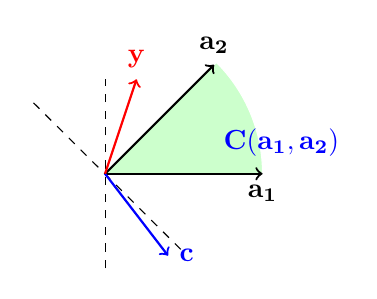
\begin{tikzpicture}[scale=0.8, auto,swap]
 
\draw[white, fill=green!20] (0,0) -- (2.5, 0) arc (0:45:2.5) -- (0,0); 
\draw[->,  thick] (0,0) -- (2.5,0) node[ultra thick, below] {$\mathbf{a_1}$};
\draw[->,  thick] (0,0) -- (1.73,1.73) node[ultra thick, above] {$\mathbf{a_2}$};
 
\draw[ dashed ] (0, -1.5) -- (0, 1.5);
\draw[ dashed ] (1.2, -1.2) -- (-1.22, 1.21);
 
\node[ thick, blue ] at (2.8, 0.5) {$\mathbf{C(a_1, a_2)}$ };
 
\draw[->, blue, thick] (0,0) -- (1, -1.3) node[ultra thick,  right ] {$\mathbf{c}$};

\draw[->, red, thick] (0,0) -- (0.5, 1.5) node[ultra thick,  above ] {$\mathbf{y}$};


         
\end{tikzpicture}
\caption{第二种情况:  $\mathbf{c} \notin \mathbf{C(a_{1}, a_{2})}$}
\end{minipage}
\end{figure}
		\subsection{引理证明}
			\paragraph{证:}
				\begin{itemize}
					\item 假如对于任意向量$\mathbf{y} \in \mathbb{R}^n$, $\mathbf{y^Ta_i\geq 0} \ (i=1,2,...,m)$,同时和任意的边界都大于等于0,即$\mathbf{y^T c \geq 0}$。那么$\mathbf{c}$一定在$\mathbf{C(a_1, a_2,..., a_m)}$中。
					\item 考虑到以下的线性规划的原始问题:
						\[
						\begin{array}{rrrrrrrrl}
 							\min & \mathbf{ c^T y } &   &\\
 							s.t. & \mathbf{ a_i^T y} & \geq& \mathbf{ 0 } & i=1,2,..., m\\
								 %      & \mathbf{ y } &\leq\geq &\mathbf{0 } \\
						\end{array} \nonumber
						\]
					\item 由于$\mathbf{ c^T y \geq 0}$,所以显然可以得到$\mathbf{ c^T y}$有一个下界为0,所以可以得到原问题的一个可行解是$\mathbf{ y=0}$。
					\item 因此可以得到他的对偶为:
						\[
						\begin{array}{rrrrrrrrl}
 							\max & 0 &  &  \\
 							s.t. & \mathbf{ x^T A^T } &=& \mathbf{c^T } \\
      							 & \mathbf{ x}  &\geq& \mathbf{0 } \\
						\end{array} \nonumber
						\]
					\item 因此我们可以得到,存在一个向量$\mathbf{ x }$使得$\mathbf{ c}=\sum_{i=1}^m x_i \mathbf{ a_i}$。所以得$\mathbf{c}$可以分解为$\mathbf{A}$的一个线性组合,即$\mathbf{c}$在$\mathbf{A}$的内部。
				\end{itemize}
			\subsection{Farkas引理变种}
				\paragraph{}Farkas引理是线性规划的核心,它可以推出很多东西,比如分离引理,博弈论里的MINMAX引理等等。
				\subsubsection{变种1}
					\paragraph{}如果$\mathbf{A}$是一个 $m\times n$的矩阵, 并且$\mathbf{b} \in \mathbb{R}^{m}$,那么可以得到:
					\begin{enumerate}
						\item $\mathbf{A x = b}$, $\mathbf{x\geq 0}$ 是一个可行解,或者
						\item 存在一个向量 $\mathbf{y}\in \mathbb{R}^{m}$ 使得 $\mathbf{y^{T} A \geq 0}$ 但是 $\mathbf{y^{T} b  < 0}$。
					\end{enumerate}
				\subsubsection{变种2}
					\paragraph{}给一些向量$\mathbf{a_1, a_{2}, ..., a_{m}} \in \mathbb{R}^n$。如果 $\mathbf{x} \in \mathbf{C(a_{1}, a_{2},..., a_{m})}$, 那么就存在一个线性堵路的向量集$\mathbf{a_1, a_{2}, ..., a_{m}}$, 对于向量集 $\mathbf{a_1, a_{2}, ..., a_{r}}$,可以得到 $\mathbf{x} \in \mathbf{C(a_{1}, a_{2},..., a_{r})}$。
				\subsubsection{变种3}
					\paragraph{}如果 $\mathbf{C} \subset \mathbb{R}^n$ 是一个闭的凸集,并且$\mathbf{x} \in \mathbb{R}^n$. 如果 $\mathbf{x} \notin \mathbf{C}$,那么肯定存在一个超平面分离 $\mathbf{x}$ 和 $\mathbf{C}$。						
	\section{对偶应用2:最短路径问题}
		\subsection{最短路径问题回顾}
			\paragraph{输入:}$n$个城市和一些道路的集合。一条从城市$i$到城市$j$的路的距离记作$d(i,j)$。两个特殊的城市:$s$和$t$。
			\paragraph{输出:}城市$s$和城市$t$之间的最短路径。
			\begin{figure}[h]
			\centering
			\begin{tikzpicture}[scale=1., auto,swap]
    			% Draw a 7,11 network
    			% First we draw the vertices
    			\foreach \pos/\name in {{(0,1.5)/s}, {(2,1)/u}, {(2,-1)/v},
                            			{(4,-1.5)/t}}
        		\node[smallvertex] (\name) at \pos {$\name$};
    			% Connect vertices with edges and draw weights
    			\foreach \source/ \dest /\weight in {s/u/5, u/t/6,u/v/1,s/v/8,          v/t/2}
        		\path[edge, blue] (\source) -- node[weight, right] {\small $\weight$} (\dest);

				%    \foreach \source/ \dest /\weight in {s/u/{x_{1}}, u/t/{x_{4}},u/v/{x_{3}},s/v/{x_{2}},          v/t/{x_{5}}}
				%        \path[edge, blue] (\source) -- node[weight, left] {$\weight$} (\dest);
				%       \draw[dashed, ->] (0,0) arc  (120:60:2);
     		\end{tikzpicture}
			\end{figure}
		\subsection{线性规划形式}
			\paragraph{}每条边我都设一个变量,可以得到以下图:
			\begin{figure}[h]
			\centering
\begin{tikzpicture}[scale=1., auto,swap]
    % Draw a 7,11 network
    % First we draw the vertices
    \foreach \pos/\name in {{(0,1.5)/s}, {(2,1)/u}, {(2,-1)/v},
                            {(4,-1.5)/t}}
        \node[smallvertex] (\name) at \pos {$\name$};
    % Connect vertices with edges and draw weights
    \foreach \source/ \dest /\weight in {s/u/5, u/t/6,u/v/1,s/v/8,          v/t/2}
        \path[edge, blue] (\source) -- node[weight, right] {\small $\weight$} (\dest);

    \foreach \source/ \dest /\weight in {s/u/{x_{1}}, u/t/{x_{4}},u/v/{x_{3}},s/v/{x_{2}},          v/t/{x_{5}}}
        \path[edge, blue] (\source) -- node[weight, left] {\small $\weight$} (\dest);
%       \draw[dashed, ->] (0,0) arc  (120:60:2);
     \end{tikzpicture}
\end{figure}
			\paragraph{}如果我用了这条边,我就让$x_i$的值等于1,没走这条边$x_i$等于0,所以可以写成一个$0/1$的线性规划,即一个整数线性规划。
			\paragraph{}写出整数线性规划方程:
				\[
				\begin{array}{rrrrrrrrrrll}
 					\min &5 x_1   &+&  8 x_2   &+& 1 x_3   &+& 6 x_4   &+& 2 x_5 & \\
 					s.t. & x_1 &+&  x_2 & &  & &   & & & = 1    & \text{向量 } s \\
      					 &     & &      & &  &-&   x_4  &-& x_5 & = -1 &\text{向量 } t  \\
      					 &  -x_1& &     &+& x_3 &+& x_4  & & & =  0  &\text{向量 } u \\
      					 &      &-& x_2 &-& x_3 & &      &+&x_5 & =  0 &\text{向量 } v  \\
      					 &   x_1 &,&     x_2 &,&    x_3  &,&    x_4  &,& x_5 & \textcolor{red}{=  0/1} 		
				\end{array} \nonumber
				\]
			\paragraph{}由于纯在全单模条件,所以可以将这个ILP问题转化成LP问题,可以得到以下的线性规划方程:
				\[
				\begin{array}{rrrrrrrrrrll}
 					\min &5 x_1   &+&  8 x_2   &+& 1 x_3   &+& 6 x_4   &+& 2 x_5 & \\
 					s.t. & x_1 &+&  x_2 & &  & &   & & & = 1    & \text{向量 } s \\
      					 &     & &      & &  &-&   x_4  &-& x_5 & = -1 &\text{向量 } t  \\
      					 &  -x_1& &     &+& x_3 &+& x_4  & & & =  0  &\text{向量 } u \\
      					 &      &-& x_2 &-& x_3 & &      &+&x_5 & =  0 &\text{向量 } v  \\
      					 &   x_1 &,&     x_2 &,&    x_3  &,&    x_4  &,& x_5 & \textcolor{red}{\geq 0} \\ 
       					 &   x_1 &,&     x_2 &,&    x_3  &,&    x_4  &,& x_5 & \textcolor{red}{\leq 1} 	
				\end{array} \nonumber
				\]
		\subsection{写出对偶问题}
			\paragraph{}通过原始问题我们可以机械的写出它的对偶问题,得到对偶的线性规划方程为:
				\[
				\begin{array}{rrrrrrrrrl}
 					\max & y_s   &-& y_t  \\
 					s.t. & y_s & &      &-& y_u & &     &  \leq 5 & \textcolor{blue}{x_{1}: \text{边 } (s,u)}  \\
      					 & y_s & &      & &     &-& y_v &  \leq 8 & \textcolor{blue}{x_{2}: \text{边 } (s,v)}   \\
     	 				 &     & &      & & y_u &-& y_v &  \leq 1 & \textcolor{blue}{x_{3}: \text{边 } (u,v)}  \\
      					 &     &-& y_t  & + & y_u & &     &  \leq 6 & \textcolor{blue}{x_{4}: \text{边 } (u,t)}  \\
      					 &     &-& y_t  & &     &+& y_v &  \leq 2 & \textcolor{blue}{x_{5}: \text{边 } (v,t)}  \\
				\end{array} \nonumber
				\]
			\paragraph{}根据下图,我们从对偶问题中可以看出,现在我们对于每个城市设一个变量$y_s$,我们用$y_s$来表示这个城市的海拔高度,$y_u$来表达另一个城市的海拔高度,现在我们知道$s$到$u$有一条路走5公里,那么他们两的海拔高度差肯定不会超过5公里,目标函数是$y_s$减去$y_t$就是$s$到$t$的最小的海拔差,我们max下它,可以得到它的下界。这就是对偶问题的直观含义。
			\begin{figure}[h]
			\centering
\begin{tikzpicture}[scale=0.8, auto,swap]
    % Draw a 7,11 network
    % First we draw the vertices
    \foreach \pos/\name in {{(0,1.5)/s}, {(2,1)/u}, {(2,-1)/v},
                            {(4,-1.5)/t}}
        \node[smallvertex] (\name) at \pos {$\name$};
    % Connect vertices with edges and draw weights
    \foreach \source/ \dest /\weight in {s/u/5, u/t/6,u/v/1,s/v/8,          v/t/2}
        \path[edge, blue] (\source) -- node[weight, right] {\small $\weight$} (\dest);

%    \foreach \source/ \dest /\weight in {s/u/{x_{1}}, u/t/{x_{4}},u/v/{x_{3}},s/v/{x_{2}},          v/t/{x_{5}}}
%        \path[edge, blue] (\source) -- node[weight, left] {$\small  \weight$} (\dest);
        
%       \draw[dashed, ->] (0,0) arc  (120:60:2);
   \draw[->, blue, thick] (-0.5, -1.75) -- (-0.5, 2); 
   \node[blue] at (-0.85, 2.2) {$height$};
   \foreach \y/\name in {-1.5/t, -1/v, 1/u, 1.5/s}
   {
   	\draw[blue, thick] (-0.55, \y) -- (-0.45, \y); 
	\node[blue]  at (-0.75, \y) {$y_\name$};
   }
   \end{tikzpicture}
   \caption{对偶问题的直观含义}
\end{figure}
	\section{对偶单纯形算法}
	\subsection{回顾原始问题单纯形算法}
		\paragraph{}原始问题:
			\[
			\begin{array}{rrrrrrrrrrrrl}
 				\min &  x_1     &+&  14 x_2    &+& 6 x_3 \\
 				s.t. &   x_1     &+&     x_2    &+& x_3 & \leq & 4   \\
      				 &   x_1     & &            & &     & \leq & 2   \\
      				 &           & &            & &  x_3& \leq & 3   \\
      				 &           & &   3x_2     &+&  x_3& \leq & 6   \\
      				 &   x_1     &,&   x_2      &,&  x_3& \geq & 0   
			\end{array} \nonumber
			\]
		\paragraph{}单纯形算法很简单,你把矩阵$\mathbf{A}$照抄下来,上面把$c$都照抄下来,$b$写在左边,初始化的最优值写左边为0,可以得到下图所示表格:
				\begin{table}[h]
				\centering
\begin{tabular}{r|rrrrrrr}\hline
  & \textcolor{black}{$x_1$} & $x_2$ & $x_3$ & \textcolor{blue}{$x_4$} & \textcolor{blue}{$x_5$} & \textcolor{blue}{$x_6$} & \textcolor{blue}{$x_7$}\\
\hline
 -z= 0 & $\overline{c_1}$= \textcolor{black}{1}  & $\overline{c_2}$=14 & $\overline{c_3}$=6 & $\overline{c_4}$=0 & $\overline{c_5}$=0 & $\overline{c_6}$=0 & $\overline{c_7}$=0 \\
 \hline
 $\mathbf{x_{B1}} = b_1'$=4 & \textcolor{black}{1} & 1 & 1 & \textcolor{blue}{1} & \textcolor{blue}{0} & \textcolor{blue}{0} & \textcolor{blue}{0} \\
 $\mathbf{x_{B2}} = b_2'$=2 & \textcolor{black}{1} & 0 & 0 & \textcolor{blue}{0} & \textcolor{blue}{1} & \textcolor{blue}{0} & \textcolor{blue}{0} \\
 $\mathbf{x_{B3}} = b_3'$=3 & \textcolor{black}{0} & 0 & 1 & \textcolor{blue}{0} & \textcolor{blue}{0} & \textcolor{blue}{1} & \textcolor{blue}{0} \\
 $\mathbf{x_{B4}} = b_4'$=6 & \textcolor{black}{0} & 3 & 1 & \textcolor{blue}{0} & \textcolor{blue}{0} & \textcolor{blue}{0} & \textcolor{blue}{1} \\
\hline
\end{tabular}
\end{table}
		\paragraph{}先找一个基可行解,所有都对他做高斯行变换,包括右边的部分都变成0。然后写一个While循环,里面分三步:
		\begin{itemize}
			\item 先找上面$c_i$内有没有负数的
			\item 有负数的话找对应的一列,在里面正的里面找最小,做高斯行变换
			\item 直到$c_i$内全是非负为止。
		\end{itemize}
		\paragraph{}最终就能得到最优解。
		\paragraph{}原始的解为$\mathbf{x}$,什么时候可行呢?即$\mathbf{x}$等于$\mathbf{B^{-1} b}$,那么$\mathbf{B^{-1} b} \geq 0$是显然的。
		\paragraph{}将线性规划写出他的对偶出来,可以得到:
			\[
			\begin{array}{rrrrrrrrrrrrl}
 				\max &  4y_1 &+&   2y_2    &+& 3y_3 &+& 6y_4&      &\\
 				s.t.    &   y_1  &+&     y_2    & &           &   &             &\leq & 1   \\
         				&   y_1  &   &               &  &          &+&  3y_4   & \leq & 14   \\
         				&   y_1   & &                &+&  y_3  &+& y_4      & \leq & 6   \\
          				&   y_1  &,&   y_2       &,&  y_3   &,&  y_4      & \leq & 0   
			\end{array} \nonumber
			\]
		\paragraph{}对应下表:
				\begin{table}[h]
				\centering
\begin{tabular}{r|rrrrrrr}\hline
  & \textcolor{black}{$x_1$} & $x_2$ & $x_3$ & \textcolor{blue}{$x_4$} & \textcolor{blue}{$x_5$} & \textcolor{blue}{$x_6$} & \textcolor{blue}{$x_7$}\\
\hline
 -z= 0 & $\overline{c_1}$= \textcolor{black}{1}  & $\overline{c_2}$=14 & $\overline{c_3}$=6 & $\overline{c_4}$=0 & $\overline{c_5}$=0 & $\overline{c_6}$=0 & $\overline{c_7}$=0 \\
 \hline
 $\mathbf{x_{B1}} = b_1'$=4 & \textcolor{black}{1} & 1 & 1 & \textcolor{blue}{1} & \textcolor{blue}{0} & \textcolor{blue}{0} & \textcolor{blue}{0} \\
 $\mathbf{x_{B2}} = b_2'$=2 & \textcolor{black}{1} & 0 & 0 & \textcolor{blue}{0} & \textcolor{blue}{1} & \textcolor{blue}{0} & \textcolor{blue}{0} \\
 $\mathbf{x_{B3}} = b_3'$=3 & \textcolor{black}{0} & 0 & 1 & \textcolor{blue}{0} & \textcolor{blue}{0} & \textcolor{blue}{1} & \textcolor{blue}{0} \\
 $\mathbf{x_{B4}} = b_4'$=6 & \textcolor{black}{0} & 3 & 1 & \textcolor{blue}{0} & \textcolor{blue}{0} & \textcolor{blue}{0} & \textcolor{blue}{1} \\
\hline
\end{tabular}
\end{table}
		\paragraph{}可以得到:
		\begin{itemize}
			\item 对偶变量是:$\mathbf{ y^T=c_B^T B^{-1} }$,可行解为$\mathbf{ y^T A}$且可行性是$\mathbf{ y^T A  \leq c^T }$。
			\item 如果一个基称为对偶可行是说$\mathbf{\overline{c^T}=c-c_B^TB^{-1}A=c^T-y^TA} \geq 0$。即只要$c_i$行都大于等于0,就是对偶可行解。
		\end{itemize}
	\subsection{从另一个角度看原始问题单纯形算法}
		\paragraph{}可以将单纯形算法看做:
		\begin{itemize}
			\item \textbf{起始点:}一开始的时候我们找一个可行解,这个可行解是$\mathbf{ x_B = B^{-1}b}$且$\mathbf{B^{-1}b \geq 0 }$。
			\item \textbf{保持:}我们在做的过程中,始终要保持左边大于等于0,原问题是可行解。
			\item \textbf{停止:}停止是最上面的$\mathbf{c_i}$行要大于等于0,即$\mathbf{ \overline{c}^T = c^T - c_B^T B^{-1} A \geq 0 }$。这个从另外一个角度看就是对偶是可行的。
		\end{itemize}
		\paragraph{}我们把我们过去的算法从对偶的观点重新再解释一遍,从一个原问题可行解出发,始终保持原问题是可行的,不断地做直到对偶也可行,一旦对偶可行我们就知道了这两者都可行了,我们就得到了最优解了。
		\paragraph{}我们也可以这样做,假如我们始终保持对偶可行,初始的数值就让对偶可行,在做的过程中始终保持对偶可行,直到最后原问题也可行,因为这两个问题都可行的话就得到最优解了,所以这么做也可以。
	\subsection{对偶单纯形算法}
	\paragraph{}通过上述的推倒,我们可以得到对偶单纯形算法为:\\
{\sc Dual simplex}$(B_I, z, \mathbf{A, b, c})$
	\begin{algorithmic}[1]
%\STATE $( B_{I}, \mathbf{A, b, c}, z)=$ {\sc InitializeSimplex}$\mathbf{(A, b, c)}$; 
\STATE \begin{footnotesize}\textcolor{blue}{//{\sc Dual simplex} starts with a dual feasible basis. Here, $B_I$ contains the indices of the basic variables.}\end{footnotesize} 
\WHILE{ \texttt{TRUE} } 
\IF{ there is no index $l$ $(1\leq l \leq m)$ has $b_{l} < 0$ }
\STATE{ $\mathbf{x}  = ${\sc CalculateX}$(B_I, \mathbf{A, b, c})$;}
\RETURN{$(\mathbf{x}, z)$};
\ENDIF;
\STATE{ choose an index $l$ having $b_{l} < 0$ according to a certain rule; }
\FOR{each index $j$ $(1\leq i \leq n)$ }
\IF{$a_{lj} < 0$} 
\STATE{ $\Delta_{j} = -\frac{c_{j}}{a_{lj}};$ } 
\ELSE
\STATE{ $\Delta_{j} = \infty;$}
\ENDIF
\ENDFOR
\STATE{choose an index $e$ that minimizes $\Delta_{j}$;} 
\IF{ $\Delta_{e} = \infty$ }
\RETURN{\texttt{''no feasible solution''};} 
\ENDIF
\STATE{$(B_{I}, \mathbf{A, b, c}, z ) = $ {\sc Pivot}$( B_{I}, \mathbf{A, b, c}, z, e, l)$;}
\ENDWHILE
\end{algorithmic}
	\subsection{例子}
	\begin{itemize}
		\item 标准型:
			\[
			\begin{array}{rrrrrrrrrrrrl}
 				\min & 5 x_1     &+&  35 x_2    &+& 20 x_3 & & \\
 				s.t.  &   x_1     &-&     x_2    &-& x_3 & \leq & -2   \\
      				  &   -x_1     &-&  3x_2     & &        & \leq & -3   \\
      				  &   x_1     &,&   x_2      &,&  x_3& \geq & 0   \\
			\end{array} \nonumber
			\]
		\item 松弛型:
			\[
			\begin{array}{rrrrrrrrrrrrl}
 				\min & 5 x_1     &+&  35 x_2    &+& 20 x_3  & &           & &                    \\
 				s.t. &   x_1     &-&     x_2    &-& x_3              &+& x_4   & &                     & = & -2   \\
      				 &   -x_1     &-&  3x_2      & &          &  &         &+& x_5              & = & -3   \\
      				 &   x_1     &,&   x_2      &,&  x_3   &, &  x_4 &,& x_5               & \geq & 0   \\
			\end{array} \nonumber
			\]
	\end{itemize}
	\subsubsection{第一步}
		\begin{table}[h]
		\centering
\begin{tabular}{r|rrrrrrr}\hline
  & \textcolor{green}{$x_1$} & $x_2$ & $x_3$ & \textcolor{blue}{$x_4$} & \textcolor{blue}{$x_5$} \\
\hline
 -z= 0 & $\overline{c_1}$= \textcolor{green}{5}  & $\overline{c_2}$=35 & $\overline{c_3}$=20 & $\overline{c_4}$=0 & $\overline{c_5}$=0  \\
 \hline
 $\mathbf{x_{B1}} = b_1'$=-2& \textcolor{green}{1} & -1   & -1 & \textcolor{blue}{1} & \textcolor{blue}{0}  \\
 $\mathbf{x_{B2}} = b_2'$=-3 & \textcolor{red}{-1} & -3 & 0  & \textcolor{blue}{0} & \textcolor{blue}{1}  \\
% $\mathbf{x_{B3}} = b_3'$=3 & \textcolor{black}{0} & 0 & 1 & \textcolor{blue}{0} & \textcolor{blue}{0} & \textcolor{blue}{1} & \textcolor{blue}{0} \\
%$\mathbf{x_{B4}} = b_4'$=6 & \textcolor{black}{0} & 3 & 1 & \textcolor{blue}{0} & \textcolor{blue}{0} & \textcolor{blue}{0} & \textcolor{blue}{1} \\
\hline
\end{tabular}
\end{table}
	\begin{itemize}
		\item 基(蓝色): $\mathbf{B =\{a_4, a_5 \} }$。
		\item 解:$\mathbf{x=\left[\begin{array}{c}\mathbf{B^{-1}b}\\\mathbf{0}\end{array}\right]}= [ 0, 0, 0, -2, -3 ]^T$。
		\item 推进:选择\textcolor{red}{$\mathbf{a_5}$}是因为 $b_2' = -3  < 0$; 选择 \textcolor{green}{$\mathbf{a_1}$}是因为 $\min_{j, a_{2j}<0} \frac{\overline{c}_j }{-a_{2j} } = \frac{ \overline{c}_1 }{-a_{21} }$。
	\end{itemize}
	\subsubsection{第二步}
		\begin{table}[h]
		\centering
\begin{tabular}{r|rrrrrrr}\hline
  & \textcolor{blue}{$x_1$} & \textcolor{green}{$x_2$} & $x_3$ & \textcolor{blue}{$x_4$} & \textcolor{black}{$x_5$} \\
\hline
 -z= -15 & $\overline{c_1}$= \textcolor{black}{0}  & $\overline{c_2}$=\textcolor{green}{20} & $\overline{c_3}$=20 & $\overline{c_4}$=0 & $\overline{c_5}$=5  \\
 \hline
 $\mathbf{x_{B1}} = b_1'$=-5& \textcolor{blue}{0} & \textcolor{red}{-4}   & -1 & \textcolor{blue}{1} & \textcolor{black}{1}  \\
 $\mathbf{x_{B2}} = b_2'$=3 & \textcolor{blue}{1} & \textcolor{green}{3} & 0  & \textcolor{blue}{0} & \textcolor{black}{-1}  \\
% $\mathbf{x_{B3}} = b_3'$=3 & \textcolor{black}{0} & 0 & 1 & \textcolor{blue}{0} & \textcolor{blue}{0} & \textcolor{blue}{1} & \textcolor{blue}{0} \\
%$\mathbf{x_{B4}} = b_4'$=6 & \textcolor{black}{0} & 3 & 1 & \textcolor{blue}{0} & \textcolor{blue}{0} & \textcolor{blue}{0} & \textcolor{blue}{1} \\
\hline
\end{tabular}
\end{table}
	\begin{itemize}
		\item 基(蓝色): \textcolor{blue}{ $\mathbf{B =\{a_1, a_4 \} }$}。
		\item 解:$\mathbf{x=\left[\begin{array}{c}\mathbf{B^{-1}b}\\\mathbf{0}\end{array}\right]}= [ 3, 0, 0, -5, 0 ]^T$。
		\item 推进: 选择 \textcolor{red}{$\mathbf{a_4}$}是因为 $b_1' = -5  < 0$; 选着 \textcolor{green}{$\mathbf{a_2}$}  是因为 $\min_{j, a_{1j}<0} \frac{\overline{c}_j }{-a_{1j} } = \frac{ \overline{c}_2 }{-a_{12} }$。
	\end{itemize}
	\subsubsection{第三步}
		\begin{table}[h]
		\centering
\begin{tabular}{r|rrrrrrr}\hline
  & \textcolor{blue}{$x_1$} & \textcolor{blue}{$x_2$} & \textcolor{green}{$x_3$} & \textcolor{black}{$x_4$} & \textcolor{black}{$x_5$} \\
\hline
 -z= -40 & $\overline{c_1}$= \textcolor{black}{0}  & $\overline{c_2}$=\textcolor{black}{0} & $\overline{c_3}$=\textcolor{green}{15} & $\overline{c_4}$=5 & $\overline{c_5}$=10  \\
 \hline
 $\mathbf{x_{B1}} = b_1'$=$\frac{5}{4}$& \textcolor{blue}{0} & \textcolor{blue}{1}   & \textcolor{green}{$\frac{1}{4}$} & \textcolor{black}{$-\frac{1}{4}$} & \textcolor{black}{$-\frac{1}{4}$}  \\
 $\mathbf{x_{B2}} = b_2'$=$-\frac{3}{4}$ & \textcolor{blue}{1} & \textcolor{blue}{0} & \textcolor{red}{$-\frac{3}{4}$}  & \textcolor{black}{$\frac{3}{4}$} & \textcolor{black}{$-\frac{1}{4}$}  \\
% $\mathbf{x_{B3}} = b_3'$=3 & \textcolor{black}{0} & 0 & 1 & \textcolor{blue}{0} & \textcolor{blue}{0} & \textcolor{blue}{1} & \textcolor{blue}{0} \\
%$\mathbf{x_{B4}} = b_4'$=6 & \textcolor{black}{0} & 3 & 1 & \textcolor{blue}{0} & \textcolor{blue}{0} & \textcolor{blue}{0} & \textcolor{blue}{1} \\
\hline
\end{tabular}
\end{table}
		\begin{itemize}
		\item 基(蓝色):textcolor{blue}{ $\mathbf{B =\{a_1, a_2 \} }$}。
		\item 解:$\mathbf{x=\left[\begin{array}{c}\mathbf{B^{-1}b}\\\mathbf{0}\end{array}\right]}= [ \frac{5}{4}, -\frac{3}{4}, 0, 0, 0 ]^T$。
		\item  推进: 选择 \textcolor{red}{$\mathbf{a_1}$} 是因为 $b_2' = -\frac{3}{4}  < 0$; 选择 \textcolor{green}{$\mathbf{a_3}$}  是因为 $\min_{j, a_{2j}<0} \frac{\overline{c}_j }{-a_{2j} } = \frac{ \overline{c}_3 }{-a_{23} }$。
	\end{itemize}
	\subsubsection{第四步}
		\begin{table}[h]
		\centering
\begin{tabular}{r|rrrrrrr}\hline
  & \textcolor{black}{$x_1$} & \textcolor{blue}{$x_2$} & \textcolor{blue}{$x_3$} & \textcolor{black}{$x_4$} & \textcolor{black}{$x_5$} \\
\hline
 -z= -55 & $\overline{c_1}$= \textcolor{black}{20}  & $\overline{c_2}$=\textcolor{black}{0} & $\overline{c_3}$=\textcolor{black}{0} & $\overline{c_4}$=20 & $\overline{c_5}$=5  \\
 \hline
 $\mathbf{x_{B1}} = b_1'$=$1$& \textcolor{black}{$\frac{1}{3}$} & \textcolor{blue}{1}   & \textcolor{blue}{0} &  \textcolor{black}{0} & \textcolor{black}{$-\frac{1}{3}$}   \\
 $\mathbf{x_{B2}} = b_2'$=$1$ & \textcolor{black}{$-\frac{4}{3}$} & \textcolor{blue}{0} & \textcolor{blue}{1}  & \textcolor{black}{-1} & \textcolor{black}{$\frac{1}{3}$}  \\
% $\mathbf{x_{B3}} = b_3'$=3 & \textcolor{black}{0} & 0 & 1 & \textcolor{blue}{0} & \textcolor{blue}{0} & \textcolor{blue}{1} & \textcolor{blue}{0} \\
%$\mathbf{x_{B4}} = b_4'$=6 & \textcolor{black}{0} & 3 & 1 & \textcolor{blue}{0} & \textcolor{blue}{0} & \textcolor{blue}{0} & \textcolor{blue}{1} \\
\hline
\end{tabular}
\end{table}
	\begin{itemize}
		\item 基(蓝色):\textcolor{blue}{ $\mathbf{B =\{a_2, a_3 \} }$}。
		\item 解:$\mathbf{x=\left[\begin{array}{c}\mathbf{B^{-1}b}\\\mathbf{0}\end{array}\right]}= [ 0, 1, 1, 0, 0 ]^T$。 
		\item 完成!
	\end{itemize}
	\subsection{对偶单纯形算法用处}
	\begin{enumerate}
		\item 对偶单纯形,如果我们原始对偶可行解好找,我们就跑对偶单纯形。很多问题我们的$\mathbf{c}$都大于等于0,那么一开始就可以找到对偶可行解,就不用一开始费劲找原始问题的可行解了。
		\item 我们日常会碰到很多的需求,比如解一个特别大的线性规划,但是解了之后别人又提了一些新要求,又要添加新约束或者更改参数,使用对偶单纯形就不用重新计算。
		\item 如果我们约束的数目比变量的数目大很多,跑对偶单纯形要好,速度非常快。
		\item 如果我们的线性规划是退化的情形,我们也要试一下对偶单纯形,这点是非常快的。
	\end{enumerate}



\section{原始对偶算法}
\subsection{原始对偶算法引入}
今天我们讲一个很重要的technique,叫原始对偶。原始对偶也是一种迭代式的,逐步改进式的迭代方法。这两节课都比较难,但是当你觉得它有用的时候,你就会觉得它不这么难了。原始对偶方法也是一种对偶方法,他也要解一个对偶。它充分利用问题的下界信息。原始对偶和原来的对偶单纯型不太一样,它不像对偶单纯型,一定要从一个对偶基可行解出发。原始对偶方法只要求对偶可行就行。第二,在原始对偶方法中,每次都要迭代解一个DRP。DRP是一个小线性规划,但很多时候,我们不用单纯型去解它。因为它有很多的直观的组合解释,尤其对于图论问题。
\subsection{原始对偶算法}


\textbf{原始对偶算法基本思路:}

我们用这幅图来说明原始对偶方法:

\begin{figure}[H]
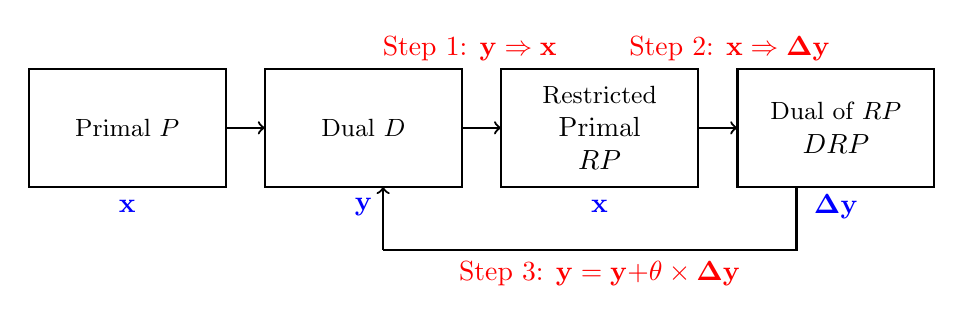
\begin{tikzpicture}[scale=1., auto,swap]

\def\l{2.5};
\def\h{1.5};
\def\d{0.5};

\draw[thick] (0,0) rectangle (\l,\h);
\draw[thick, ->] (\l, \h*0.5) -- ( \l + \d, \h*0.5);
\node[ultra thick] at (\l*0.5, \h*0.5) {\small Primal $P$};
\node[thick, blue] at (\l*0.5 , -0.25) {$\mathbf{x}$};

\node[thick, red] at (\l + \d + \l + \d*0.2 , \h + 0.25 ) {Step $1$: $\mathbf{y\Rightarrow x}$};


\draw[thick] (0 + \l + \d, 0) rectangle (\l + \l + \d,\h);
\draw[thick, ->] (\l + \l + \d , \h*0.5) -- ( \l + \d + \l + \d, \h*0.5);
\node[ultra thick] at (\l+\d + \l*0.5, \h*0.5) {\small Dual  $D$};
\node[thick, blue] at (\l+\d + \l*0.5, -0.25) {$\mathbf{y}$};

\node[thick, red] at (\l + \d + \l + \d + \l + \d*0.8 , \h + 0.25 ) {Step $2$: $\mathbf{x}\Rightarrow \mathbf{\Delta y}$};


\draw[thick] (0 + \l + \d + \l + \d, 0) rectangle (\l + \l + \d+ \l + \d,\h);
\draw[thick, ->] (\l + \l + \d + \l + \d, \h*0.5) -- ( \l + \d + \l + \d + \l + \d, \h*0.5);
\node[ultra thick, align=center] at (\l+\d + \l+\d + \l*0.5,  \h*0.5) {\small Restricted\\ Primal\\ $RP$};
\node[thick, blue] at (\l+\d + \l+\d + \l*0.5,  -0.25) {$\mathbf{x}$};

\node[thick, red] at (\l+\d + \l+\d + \l*0.5,  -1.1) { Step $3$: $\mathbf{y = y + }\theta \times \mathbf{\Delta y}$};


\draw[thick] (0 + \l + \d + \l + \d + \l + \d, 0) rectangle (\l + \l + \d+ \l + \d + \l + \d,\h);
\node[ultra thick, align=center] at (\l+\d + \l+\d + \l+\d + \l*0.5 , \h*0.5) {\small Dual of $RP$\\ $DRP$};
\node[thick, blue] at (\l+\d + \l+\d + \l+\d + \l*0.5 , -0.25) {$\mathbf{\Delta y}$};

\draw[thick] (\l+\d + \l+\d + \l+\d + \l*0.3 , 0) -- (\l+\d + \l+\d + \l+\d + \l*0.3 , -0.8) -- (\l+\d + \l*0.6, -0.8);
\draw[thick, ->]  (\l+\d + \l*0.6, -0.8) --  (\l+\d + \l*0.6, 0);


\end{tikzpicture}
\end{figure}

假如我们要求解远线性规划问题P,它的变量是X。我们先把它的对偶问题写出来。假如我们拿到对偶问题的一个可行解Y,我们把Y带入到对偶问题中,看看Y能指导我们得到X多少的信息,得到的X的信息又能够知道我们如何改进Y。通过这样不断迭代改进Y,找到最优解。这里有很多名词,大家先不要着急,一个个的看下去。


\textbf{得到RP}

看个例子。
\begin{itemize}
\begin{footnotesize}
\item
Primal P:
\[
\begin{array}{rrrrrrrrrrrrl}
 \min & c_1x_1    &+&  c_2x_2   &+&  ...&+& c_nx_n    &      &    & \\
 s.t. & a_{11}x_1 &+& a_{12}x_2 &+& ... &+& a_{1n}x_n & = & b_1 & \textcolor{blue}{(y_1)} \\
      & a_{21}x_1 &+& a_{22}x_2 &+& ... &+& a_{2n}x_n & = & b_2 & \textcolor{blue}{(y_2)} \\
      &           & &           & & ... & &           &      &     &  \\
      & a_{m1}x_1 &+& a_{m2}x_2 &+& ... &+& a_{mn}x_n & = & b_m &  \textcolor{blue}{(y_m)}\\
      &       x_1 &,&       x_2 &,& ... &,&       x_n & \geq & 0   &  \\
     \end{array} \nonumber
\]
\item
Dual D:
\[
\begin{array}{rrrrrrrrrrrrl}
 \max & b_1y_1    &+&  b_2y_2   &+&  ...&+& b_my_m    &      &    & \\
 s.t. & a_{11}y_1 &+& a_{21}y_2 &+& ... &+& a_{m1}y_m & \leq & c_1 &  \\
      & a_{12}y_1 &+& a_{22}y_2 &+& ... &+& a_{m2}y_m & \leq & c_2 &  \\
      &           & &           & & ... & &           &      &     &  \\
      & a_{1n}y_1 &+& a_{2n}y_2 &+& ... &+& a_{mn}y_m & \leq & c_n &
%      &       y_1 &,&       y_2 &,&     &,&       y_m & \leq\geq & 0   & \\
     \end{array} \nonumber
\]
\end{footnotesize}
\end{itemize}
原始问题如上所示,我们将它的对偶问题写出来。怎么写对偶呢,我们再重复一遍。对偶就是拉格朗日乘子,每一行的约束做一个拉格朗日乘子,就是变量,叫做y1,y2,……。然后写出对偶问题。

假如我们拿到了对偶问题的一个可行解y,我们首先验证y是不是最优解。如何验证呢?

首先,如果y是最优解,则x要满足一个条件。什么条件呢?就是这样一个条件:
\begin{itemize}
\begin{small}

\item Dual problem D:
\[
\begin{array}{rrrrrrrrrrrrl}
\max & b_1y_1    &+&  b_2y_2   &+&  ...&+& b_my_m    &      &    & \\
 s.t. & a_{11}y_1 &+& a_{21}y_2 &+& ... &+& a_{m1}y_m & \leq & c_1 &  \textcolor{blue}{('='\Rightarrow x_1 \geq 0 )} \\
      %& a_{12}y_1 &+& a_{22}y_2 &+& ... &+& a_{m2}y_m & \leq & c_2 &  ('='\Rightarrow x_2 \geq 0 )\\
      &           & &           & & ... & &           &      &     &  \\
      & a_{1n}y_1 &+& a_{2n}y_2 &+& ... &+& a_{mn}y_m & \leq & c_n &  \textcolor{blue}{ ('<'\Rightarrow x_n = 0 )}
%      &       y_1 &,&       y_2 &,&     &,&       y_m & \leq\geq & 0   & \\
     \end{array} \nonumber
\]
\end{small}
\end{itemize}
假如我们拿到一个y,我们把y带入对偶问题的约束中,对于每一条约束,如果约束1取等号,则相当于没有告诉我x1的任何信息,x1大于等于0是本来就已知的。如果约束n取小于号,大家回忆一下我们讲的互补松弛性,如果约束取小于,xn必定等于0。
我们用$J$表示满足等于号的约束:
 \begin{figure}[H]
 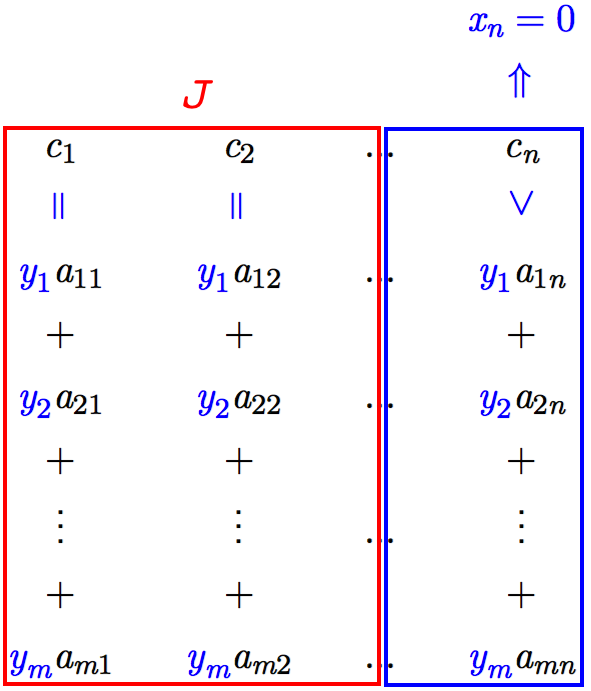
\includegraphics[width=2.5in] {L9-RP.png}
\end{figure}
我们回到原始问题,如果Y是一个最优解,那么红框内表示满足的等号约束,篮框内的取小于号,对应的xn=0。也就是说给我一个Y,如果是最优的,带进去,X必须要满足这些条件:
\begin{itemize}
\begin{small}
\item RP:
\[
\begin{array}{rrrrrrrrrrrrl}
 %\min & 0& \\
      & a_{11}x_1 &+& a_{12}x_2 &+& ... &+& a_{1n}x_n & = & b_1 &  \\
      & a_{21}x_1 &+& a_{22}x_2 &+& ... &+& a_{2n}x_n & = & b_2 & \\
      &           & &           & & ... & &           &      &     &  \\
      & a_{m1}x_1 &+& a_{m2}x_2 &+& ... &+& a_{mn}x_n & = & b_m & \\
      &           & &           & &     & &       \textcolor{blue}{x_i} & \textcolor{blue}{=} & 0   &\textcolor{blue}{ i\notin J} \\
      &           & &           & &     & &       \textcolor{red}{x_i} & \textcolor{red}{\geq} & 0   & \textcolor{red}{i\in J}
     \end{array} \nonumber
\]
\end{small}
\end{itemize}
我们只需要解这个限制性的原问题restricted primal (RP)就可以了。没有目标函数,只需要X满足这些约束就够了。
解这个不等式约束问题,我们把它转化成线性规划问题来做。加一些松弛变量:s1,s2,...,sm,变成下面这样一个问题:
\[
\begin{array}{rrrrrrrllllllllll}
 \min &\epsilon=&s_1    &+s_2   &...&+s_{m} &                   &    &                     &        & \\
 s.t.   &               &s_1    &           &   &            &+a_{11}x_1 &... &+a_{1n}x_{n} & =b_1 & \\
         &               &         &  s_2    &   &            &+a_{21}x_1 &... &+a_{2n}x_{n} & =b_2 & \\
         &               &         &           &...&            &                    &... &                     &          &\\
         &               &         &           &   & s_m    &+a_{m1}x_1 &... &+a_{mn}x_{n} & =b_m & \\
         &               &         &           &    &            &                         &   &\textcolor{blue}{x_i} & \textcolor{blue}{=  0}   &\textcolor{blue}{ i\notin J} \\
         &               &         &           &    &            &                         &    &\textcolor{red}{x_i}  &       \textcolor{red}{\geq  0}   & \textcolor{red}{i\in J} \\
         &               &         &           &     &            &                        &    &             s_i     & \geq 0 &  \forall i  \\
     \end{array} \nonumber
\]
最优值如果等于0,表明我们能找到一个X满足RP。如果最优值大于0,RP没有可行解,所以Y就不是最优解。


\textbf{如何求解RP:DRP}

现在,我们回顾一下。如果Y是最优解,对应的X满足原先的约束,并且有些Xi=0(蓝框内)。我们只要找到这些X,Y就是最优的。如何找这些X呢?求解RP对应的线性规划,当然,我们不一定需要直接去解RP对应的线性规划,我们解RP对应的线性规划的对偶($DRP$),也是等价的:
\begin{itemize}
\item $DRP$:
\[
\begin{array}{rrrrrrrrrrrrrrrrrrrrl}
\max & w &=& b_1y_1    &+&  b_2y_2   &+&  ...&+& b_my_m    &      &    & \\
 s.t. & & & a_{11}y_1 &+& a_{21}y_2 &+& ... &+& a_{m1}y_m & \leq & 0 &  \\
      & & & a_{12}y_1 &+& a_{22}y_2 &+& ... &+& a_{m2}y_m & \leq & 0 &  \\
      & & &          & &           & & ... & &           &      &     &  \\
      & & & a_{1|J|}y_1 &+& a_{2|J|}y_2 &+& ... &+& a_{m|J|}y_m & \leq & 0 & \\
      & & &      y_1 &,&       y_2 &,&     &,&       y_m & \leq & 1   & \\
     \end{array} \nonumber
\]
\end{itemize}
当最优值是0的时候,Y就是最优的。否则Y不是最优的。当Y不是最优时,应该怎么办。这个时候虽然Y不是最优,但是我们对这个问题的求解所花的功夫没有白费。它提供了有用的信息,它可以告诉我们怎么改进Y。


\textbf{DRP优化y}

为什么说我们求得的DRP的解可以改进Y的呢?
我们构造一个解:$\mathbf{y' = y +} \theta \mathbf{ \Delta y}, \theta > 0 $.
如果说它要是改进的话,我们只要理解两点。第一点目标函数的确是变大啦。第二点,y是满足约束的,y'也应该是满足约束的。

我们先看第一点。DRP问题的目标函数和对偶问题的目标函数是一样的。所以,如果DRP问题的目标函数能找到一个最优解,它是等于0的,那我们就已经stop了,如果是大于0的话,我们可以知道,$\mathbf{\Delta y^T b } = w_{OPT}  > 0$,  $\mathbf{y'^T b = y^T b } + \theta w_{OPT}  > \mathbf{ y^T b}$.

第二点,y本来是满足约束的,会不会变大以后就不满足约束了呢。
对于任意的$ j \in J$,  $a_{1j} \Delta y_1 + a_{2j}\Delta y_2 + ... + a_{mj}\Delta y_m  \leq  0$(依据DRP的约束). 所以我们有 $\mathbf{y'^Ta_j} = \mathbf{y^Ta_j} + \theta \mathbf{\Delta y^Ta_j} \leq \mathbf{c_j}$ 对于任意的 $\theta > 0$.
对于$j \notin J$,又分两种情况:

第一种,对于$\forall j \notin J, a_{1j} \Delta y_1 + a_{2j}\Delta y_2 + ... + a_{mj}\Delta y_m  \leq  0$:

$\mathbf{y'}$肯定是一个可行解,对于 $\forall \theta > 0$ ,$\forall 1 \leq j \leq n$:
 \begin{eqnarray}
&&  a_{1j}y'_1 + a_{2j}y'_2 + ... + a_{mj}y'_m \\
&=&a_{1j}y_1 + a_{2j}y_2 + ... + a_{mj}y_m \\
&+&\theta(a_{1j}\Delta{y_1} + a_{2j}\Delta{y_2} + ... + a_{mj}\Delta{y_m}) \\
&\leq& c_j
\end{eqnarray}
换句话说,对偶问题是无界的,原问题是不可行的。因为原问题的解可以任意大。

第二种,$\exists j \notin J, a_{1j} \Delta y_1 + a_{2j}\Delta y_2 + ... + a_{mj}\Delta y_m  >  0$:

我们可以设置$\theta \leq \frac{c_j - (a_{1j}y_1 + a_{2j}y_2 + ... + a_{mj}y_m) } {a_{1j}\Delta {y_1} + a_{2j}\Delta {y_2} + ... + a_{mj}\Delta {y_m}} = \frac{ \mathbf{c_j - y^Ta_j} }{ \mathbf{\Delta y^T a_j}  }$ 从而使得$\mathbf{y'^Ta_j} =\mathbf{y^Ta_j} + \theta \mathbf{\Delta y^Ta_j} \leq \mathbf{c_j}$.


\textbf{原始对偶算法}

讲完这些,原始对偶算法就出来啦:
\begin{itemize}
\item 原始对偶算法:
\begin{small}
\begin{algorithmic} [1]
\STATE Infeasible = ``No''\\
       Optimal = ``No''\\
        $\mathbf{y=y_{0}}$; \qquad //$\mathbf{y_{0}}$ is a feasible solution to the dual problem $D$
\WHILE{TRUE}
\STATE Finding tight constraints index $J$, and set corresponding $x_j = 0 $ for $ j\notin J$.
\STATE Thus we have a smaller RP.
\STATE Solve DRP. Denote the solution as $\Delta \mathbf{y}$.
\IF{DRP objective function $w_{OPT} =0$}
\STATE Optimal=``Yes''\\
\RETURN $y$;
\ENDIF
\IF{ $\mathbf{\Delta y^T a_j \leq 0} $ (for all $j \notin J$)}
\STATE Infeasible = ``Yes'';
\RETURN;
\ENDIF
\STATE Set $\theta = \min{ \frac{ \mathbf{c_j - y^Ta_j} }{ \mathbf{\Delta y^T a_j}}}$ for $\mathbf{\Delta y^T a_j}>0$, $j\notin J$.
\STATE Update $\mathbf{ y}$ as  $ \mathbf{ y = y + \theta \Delta y}$;
\ENDWHILE
\end{algorithmic}
\end{small}
\end{itemize}
下面我们看一下原始对偶算法的优点。

1. 原始对偶算法肯定会结束。如果用一些防止退化的规则的话,肯定会结束的。(如何使用Bland法则防止退化的slides放到了网上)

2. 我们会看到无论是RP还是DRP都不显式的依赖于c。实际上那个c已经表达在那个J当中了。J就是我们得到的那些约束。

这就导致了原始对偶算法的一个很重要的优点。那就是:RP经常是一个纯粹性的组合问题。在最短路径问题当中,RP可以直接转化为一个组合问题--连通可达性问题。
我们把一个可行解带到对偶问题后,约束域的约束分成了两部分。一部分约束取等于号(我们看到的图中的红框);另一部分取严格小于号(图中的蓝框),这一部分对应的Xi=0,这意味着这些约束将不需要再考虑。问题的规模一下子大大缩小。我们只需要考虑红框的问题。原始对偶的优势就在于,每次都把问题缩小一块儿。
我们现在比较一下对偶问题和DRP问题:
\begin{itemize}
\item 对偶问题:
\[
\begin{array}{rrrrrrrrrrrrl}
\max & b_1y_1    &+&  b_2y_2   &+&  ...&+& b_my_m    &      &    & \\
 s.t. & a_{11}y_1 &+& a_{21}y_2 &+& ... &+& a_{m1}y_m & \leq & c_1 &   \\
      & a_{12}y_1 &+& a_{22}y_2 &+& ... &+& a_{m2}y_m & \leq & c_2 & \\
      &           & &           & & ... & &           &      &     &  \\
      & a_{1n}y_1 &+& a_{2n}y_2 &+& ... &+& a_{mn}y_m & \leq & c_n &
%      &       y_1 &,&       y_2 &,&     &,&       y_m & \leq\geq & 0   & \\
     \end{array} \nonumber
\]
\item DRP:
\[
\begin{array}{rrrrrrrrrrrrrrrrrrrrl}
\max & w &=& b_1y_1    &+&  b_2y_2   &+&  ...&+& b_my_m    &      &    & \\
 s.t. & & & a_{11}y_1 &+& a_{21}y_2 &+& ... &+& a_{m1}y_m & \leq & \textcolor{red}{0} &  \\
      & & & a_{12}y_1 &+& a_{22}y_2 &+& ... &+& a_{m2}y_m & \leq & \textcolor{red}{0} &  \\
      & & &          & &           & & ... & &           &      &     &  \\
      & & & a_{1\textcolor{red}{|J|}}y_1 &+& a_{2\textcolor{red}{|J|}}y_2 &+& ... &+& a_{m\textcolor{red}{|J|}}y_m & \leq & \textcolor{red}{0} & \\
      & & &      y_1 &,&       y_2 &,&     &,&       y_m & \leq & \textcolor{red}{1}   & \\
     \end{array} \nonumber
\]
\end{itemize}
非常好的形式,DRP的目标函数和对偶问题一模一样。约束有三点不一样,第一个,约束不再是小于等于ci了,而是小于等于0。第二点,只需要管红框里的约束,蓝框里的不用管了。第三点,每个yi都小于等于1
们可以总结下如果要用动态规划的算法去解决实际问题,需要有哪些要素、解决问题的关键是什么以及怎样描述并定义子问题。
\subsection{最短路径: Dijkstra's algorithm基本上是原始对偶算法}
我们再回顾一下 Dijkstra's algorithm,我们说它不适合第一节课学,因为他他太精巧,太聪明了,而我们很难从中学到东西。
现在我们对这个问题跑一下原始对偶。原始对偶是一个套路。假如要求一个原始问题P,我们可以很机械的把它的对偶问题D写出来。然后我们把一个Y带进去,直接求出针对这个Y的DRP。如果DRP求出的解是0,那就是最优解,如果大于0,则更新Y,不断重复。这么一个机械性的东西竟然就是 Dijkstra's algorithm。


\textbf{最短路径问题}

我们看一下这个最短路径问题,四个城市:s,u,v,t。城市之间有路连接,求最短路径。
\begin{figure}[H]
\begin{tikzpicture}[scale=1., auto,swap]
    % Draw a 7,11 network
    % First we draw the vertices
    \foreach \pos/\name in {{(0,1.5)/s}, {(2,1)/u}, {(2,-1)/v},
                            {(4,-1.5)/t}}
        \node[smallvertex] (\name) at \pos {$\name$};
    % Connect vertices with edges and draw weights
    \foreach \source/ \dest /\weight in {s/u/5, u/t/6,u/v/1,s/v/8,          v/t/2}
        \path[edge, blue] (\source) -- node[weight, right] {\small $\weight$} (\dest);

%    \foreach \source/ \dest /\weight in {s/u/{x_{1}}, u/t/{x_{4}},u/v/{x_{3}},s/v/{x_{2}},          v/t/{x_{5}}}
%        \path[edge, blue] (\source) -- node[weight, left] {$\weight$} (\dest);
%       \draw[dashed, ->] (0,0) arc  (120:60:2);
     \end{tikzpicture}
\end{figure}


\textbf{最短路径问题的对偶以及简化}

写出它的原始线性规划:
\begin{small}
\[
\begin{array}{rrrrrrrrrrll}
 \min &5 x_1   &+&  8 x_2   &+& 1 x_3   &+& 6 x_4   &+& 2 x_5 & \\
 s.t. & x_1 &+&  x_2 & &  & &   & & & = 1    & \text{vertex } s \\
      &     & &      & &  &-&   x_4  &-& x_5 & = -1 &\text{vertex } t  \\
      &  -x_1& &     &+& x_3 &+& x_4  & & & =  0  &\text{vertex } u \\
      &      &-& x_2 &-& x_3 & &      &+&x_5 & =  0 &\text{vertex } v  \\
      &   x_1 &,&     x_2 &,&    x_3  &,&    x_4  &,& x_5 & \textcolor{red}{\geq 0} \\
       &   x_1 &,&     x_2 &,&    x_3  &,&    x_4  &,& x_5 & \textcolor{red}{\leq 1} 	
\end{array} \nonumber
\]
\end{small}
对于约束条件,我们要求xi应该取0或者1。如果这样的话,问题挺难的。对于这个问题,我们可以松弛一下,变成大于等于0小于等于1.由于全单模条件,这两个条件的解是一样的。

写出原问题的对偶:
\begin{small}
\[
\begin{array}{rrrrrrrrrl}
 \max & y_s   &-& y_t  \\
 s.t. & y_s & &      &-& y_u & &     &  \leq 5 & \textcolor{blue}{x_{1}: \text{edge } (s,u)}  \\
      & y_s & &      & &     &-& y_v &  \leq 8 & \textcolor{blue}{x_{2}: \text{edge } (s,v)}   \\
      &     & &      & & y_u &-& y_v &  \leq 1 & \textcolor{blue}{x_{3}: \text{edge } (u,v)}  \\
      &     &-& y_t  & + & y_u & &     &  \leq 6 & \textcolor{blue}{x_{4}: \text{edge } (u,t)}  \\
      &     &-& y_t  & &     &+& y_v &  \leq 2 & \textcolor{blue}{x_{5}: \text{edge } (v,t)}  \\
\end{array} \nonumber
\]
\end{small}
原问题相当于对每个边设一个变量,对偶问题相当于对城市设置变量。yi可以理解为城市i的海拔高度。优化目标为ys-yt,是原问题的下边界。求它的最大值。
\begin{figure}[H]
\begin{tikzpicture}[scale=0.8, auto,swap]
    % Draw a 7,11 network
    % First we draw the vertices
    \foreach \pos/\name in {{(0,1.5)/s}, {(2,1)/u}, {(2,-1)/v},
                            {(4,-1.5)/t}}
        \node[smallvertex] (\name) at \pos {$\name$};
    % Connect vertices with edges and draw weights
    \foreach \source/ \dest /\weight in {s/u/5, u/t/6,u/v/1,s/v/8,          v/t/2}
        \path[edge, blue] (\source) -- node[weight, right] {\small $\weight$} (\dest);

%    \foreach \source/ \dest /\weight in {s/u/{x_{1}}, u/t/{x_{4}},u/v/{x_{3}},s/v/{x_{2}},          v/t/{x_{5}}}
%        \path[edge, blue] (\source) -- node[weight, left] {$\small  \weight$} (\dest);

%       \draw[dashed, ->] (0,0) arc  (120:60:2);
   \draw[->, blue, thick] (-0.5, -1.75) -- (-0.5, 2);
   \node[blue] at (-0.85, 2.2) {$height$};
   \foreach \y/\name in {-1.5/t, -1/v, 1/u, 1.5/s}
   {
   	\draw[blue, thick] (-0.55, \y) -- (-0.45, \y);
	\node[blue]  at (-0.75, \y) {$y_\name$};
   }
   \end{tikzpicture}
\end{figure}

跑原始对偶算法,首先简化原始问题,将yt固定为0。问题变为:
\begin{small}
\[
\begin{array}{rrrrrrrrrl}
 \max & y_s   & &   \\
 s.t. & y_s & &      &-& y_u & &     &  \leq 5 & \textcolor{blue}{x_{1}: \text{edge } (s,u)}  \\
      & y_s & &      & &     &-& y_v &  \leq 8 & \textcolor{blue}{x_{2}: \text{edge } (s,v)}   \\
      &     & &      & & y_u &-& y_v &  \leq 1 & \textcolor{blue}{x_{3}: \text{edge } (u,v)}  \\
      &     & &    &   & y_u & &     &  \leq 6 & \textcolor{blue}{x_{4}: \text{edge } (u,t)}  \\
      &     & &   & &     & & y_v &  \leq 2 & \textcolor{blue}{x_{5}: \text{edge } (v,t) } \\
\end{array} \nonumber
\]
\end{small}


\textbf{第一次迭代}

设置一个初始可行解: $\mathbf{y^T} = (0, 0, 0)$.将其带入约束,判断哪些约束取等号,哪些取不等。根据互补松弛性,确定哪些xi=0。
 \begin{small}
\[
\begin{array}{rrrrrrrrrrl}
 & y_s & &      &-& y_u & &     &  \textcolor{blue}{<}& 5 &  \textcolor{blue}{\Rightarrow  x_{1}  = 0}   \\
 & y_s & &      & &     &-& y_v &   \textcolor{blue}{<}&  8 & \textcolor{blue}{\Rightarrow  x_{2}  = 0}  \\
  &     & &      & & y_u &-& y_v &   \textcolor{blue}{<}&  1 & \textcolor{blue}{\Rightarrow  x_{3}  = 0} \\
 &     & &    &   & y_u & &     &   \textcolor{blue}{<}&  6 & \textcolor{blue}{\Rightarrow  x_{4}  = 0}  \\
 &     & &   & &     & & y_v &   \textcolor{blue}{<}&  2 & \textcolor{blue}{\Rightarrow  x_{5}  = 0}
\end{array} \nonumber
\]
\end{small}
验证可知在$D$中, \textcolor{red}{$J=\Phi$},即 $x_2,x_3,x_4,x_5=0$。

把当前的RP写出来:
\[
\begin{array}{rrrrrrrrrrrrrrrrrl}
 \min & s_1 &+s_2 & +s_3 &     &        &    &     &   & \\
 s.t. & s_1 &     &     & \textcolor{blue}{+x_1}  & \textcolor{blue}{+x_2} &    &     &   & = 1    & \text{node }s  \\
%       &     & &      & &  &-&   x_4  &-& x_5 & = -1 &\text{vertex t}  \\
     &      &s_2     &             &  \textcolor{blue}{-x_1}  &     & \textcolor{blue}{+x_3}  &  \textcolor{blue}{+x_4}     &  & =  0  & \text{node }u\\
     &      &          & s_3       &     & \textcolor{blue}{-x_2}    & \textcolor{blue}{-x_3}  &      & \textcolor{blue}{+x_5} & =  0 & \text{node }v \\
     & s_1, &s_2, &s_3,  &      &          &         &         &     & \geq 0 \\
     &         &       &         &  \textcolor{blue}{x_1,} &    \textcolor{blue}{ x_2,} &    \textcolor{blue}{x_3,} &   \textcolor{blue}{x_4,} & \textcolor{blue}{x_5} & \textcolor{blue}{= 0} \\ 	
\end{array} \nonumber
\]
蓝色的xi是为了突出表示xi=0。

写出DRP:
\[
\begin{array}{rrrrrrrrrl}
 \max & y_s &      & &            &\\
s.t. & y_s  &      & &     \leq 1 &  \\
     &      & y_u  & &     \leq 1 &  \\
     &      &      & & y_v \leq 1 &  \\
\end{array} \nonumber
\]
如果原先的$\mathbf{y}$(0,0,0)是最优解的话,对应的$x$一定满足RP, $\Delta \mathbf{y}$满足DRP.

原始对偶算法应用到图论上,常常是这样的:写出的线性规划,对应的DRP形式很特殊,解能够很明显的看出来。

采用组合技术求解$DRP$,通过DRP求解,可以知道当前的y不是最优。对于DRP的最优值,找一个最优解 $\Delta \mathbf{y^T} = (1, 0, 0)$。(最优解不唯一)

计算步长$\theta$: $\theta = \min \{ \frac{ \mathbf{c_1 - y^Ta_1} }{ \mathbf{\Delta y^T a_1}  }, \frac{ \mathbf{c_2 - y^Ta_2} }{ \mathbf{\Delta y^T a_2}  }  \} = \min\{ 5, 8\} = 5$

更新 $\mathbf{y}$: $\mathbf{y^T=y^T}+\theta \Delta \mathbf{y^T}  = (5, 0, 0)$.

经过一次迭代更新以后,城市之间的状态如图:
\begin{figure}[H]
\begin{tikzpicture}[scale=0.8, auto,swap]

    \def\ys{2};
    \def\yu{0};
    \def\yv{0};
    \def\yt{0};

    \foreach \pos/\name in {{(0,\ys)/s}, {(0,\yu)/u}, {(1.3,\yv)/v}, {(3,\yt)/t}}
        \node[smallvertex] (\name) at \pos {$\name$};

    \foreach \source/ \dest /\weight in {s/u/5,s/v/8}
        \path[edge, blue] (\source) -- node[weight, right] {\small $\weight$} (\dest);
    \foreach \source/ \dest /\weight in { u/v/1, v/t/2}
        \path[edge, blue] (\source) -- node[weight, below] {\small $\weight$} (\dest);
    \draw[->, thick, blue] (u) to[out=-60, in=240] node[below]{\small $6$} (t);

   \draw[->, blue, thick] (-0.5, -0.2) -- (-0.5, 2.3);
   \node[blue] at (-1.2, 2.5) {$height$};

    	\draw[blue, thick] (-0.55, \yu) -- (-0.45, \yu);
	\node[blue]  at (-2.3, \yu) {$y_u=y_v=y_t=0$};

    	\draw[blue, thick] (-0.55, \ys) -- (-0.45, \ys);
	\node[blue]  at (-1.2, \ys) {$y_s=5$};

   \end{tikzpicture}
\end{figure}

我们就拿这一步来看,为什么说原始对偶算法就是Dijkstra's algorithm。

从Dijkstra's algorithm的角度来看:

DRP的最优解:$\Delta \mathbf{y^T} = (1, 0, 0)$,对应着Dijkstra's algorithm滴墨水的起始位置,也是被染的点集合$S = \{s\}$。第一次的最优解对应染的第一个点。DRP的实际目的找到墨水所要染的点。

步长 $\theta = \min \{ \frac{ \mathbf{c_1 - y^Ta_1} }{ \mathbf{\Delta y^T a_1}  }, \frac{ \mathbf{c_2 - y^Ta_2} }{ \mathbf{\Delta y^T a_2}  }  \} = \min\{ 5, 8\} = 5$:对于现在墨水所染得点集合 $S$ ,下一次墨水能染的最短距离。


\textbf{第二次迭代}

将新的可行解 $\mathbf{ y^T = (5, 0, 0) }$带入,检查约束:
 \begin{small}
\[
\begin{array}{rrrrrrrrrrl}
 & y_s & &      &-& y_u & &     &  \textcolor{red}{=}& 5 &  \\
 & y_s & &      & &     &-& y_v &   \textcolor{blue}{<}&  8 & \textcolor{blue}{\Rightarrow  x_{2}  = 0}  \\
  &     & &      & & y_u &-& y_v &   \textcolor{blue}{<}&  1 & \textcolor{blue}{\Rightarrow  x_{3}  = 0} \\
 &     & &    &   & y_u & &     &   \textcolor{blue}{<}&  6 & \textcolor{blue}{\Rightarrow  x_{4}  = 0}  \\
 &     & &   & &     & & y_v &   \textcolor{blue}{<}&  2 & \textcolor{blue}{\Rightarrow  x_{5}  = 0}
\end{array} \nonumber
\]
\end{small}
可知在$D$中:  \textcolor{red}{$J=\{ 1\}$}, 即 $x_2,x_3,x_4,x_5=0$.

对应的RP:
\[
\begin{array}{rrrrrrrrrrrrrrrrrl}
 \min & s_1 &+s_2 & +s_3 &     &        &    &     &   & \\
 s.t. & s_1 &     &     & \textcolor{blue}{+x_1}  & \textcolor{blue}{+x_2} &    &     &   & = 1    & \text{node }s  \\
%       &     & &      & &  &-&   x_4  &-& x_5 & = -1 &\text{vertex t}  \\
     &      &s_2     &             &  \textcolor{blue}{-x_1}  &     & \textcolor{blue}{+x_3}  &  \textcolor{blue}{+x_4}     &  & =  0  & \text{node }u\\
     &      &          & s_3       &     & \textcolor{blue}{-x_2}    & \textcolor{blue}{-x_3}  &      & \textcolor{blue}{+x_5} & =  0 & \text{node }v \\
     & s_1, &s_2, &s_3,  &      &          &         &         &     & \geq 0 \\
     &         &       &         &  \textcolor{blue}{x_1,} &    \textcolor{blue}{ x_2,} &    \textcolor{blue}{x_3,} &   \textcolor{blue}{x_4,} & \textcolor{blue}{x_5} & \textcolor{blue}{= 0} \\ 	
\end{array} \nonumber
\]

写出DRP:
\[
\begin{array}{rrrrrrrrrl}
 \max & y_s &      & &            &\\
s.t. & y_s  &      & &     \leq 1 &  \\
     &      & y_u  & &     \leq 1 &  \\
     &      &      & & y_v \leq 1 &  \\
\end{array} \nonumber
\]

采用组合技术求解$DRP$,通过DRP求解,可以知道当前的y不是最优。对于DRP的最优值,找一个最优解 $\Delta \mathbf{y^T} = (1, 0, 0)$。(最优解不唯一)
步长$\theta$: $\theta = \min \{ \frac{ \mathbf{c_1 - y^Ta_1} }{ \mathbf{\Delta y^T a_1}  }, \frac{ \mathbf{c_2 - y^Ta_2} }{ \mathbf{\Delta y^T a_2}  }  \} = \min\{ 5, 8\} = 5$。

更新$\mathbf{y}$: $\mathbf{y^T=y^T}+\theta \Delta \mathbf{y^T}  = (5, 0, 0)$.

经过第二次迭代更新以后,城市之间的状态如图:
\begin{figure}[H]
\begin{tikzpicture}[scale=0.8, auto,swap]

    \def\ys{2};
    \def\yu{0};
    \def\yv{0};
    \def\yt{0};

    \foreach \pos/\name in {{(0,\ys)/s}, {(0,\yu)/u}, {(1.3,\yv)/v}, {(3,\yt)/t}}
        \node[smallvertex] (\name) at \pos {$\name$};

    \foreach \source/ \dest /\weight in {s/u/5,s/v/8}
        \path[edge, blue] (\source) -- node[weight, right] {\small $\weight$} (\dest);
    \foreach \source/ \dest /\weight in { u/v/1, v/t/2}
        \path[edge, blue] (\source) -- node[weight, below] {\small $\weight$} (\dest);
    \draw[->, thick, blue] (u) to[out=-60, in=240] node[below]{\small $6$} (t);

   \draw[->, blue, thick] (-0.5, -0.2) -- (-0.5, 2.3);
   \node[blue] at (-1.2, 2.5) {$height$};

    	\draw[blue, thick] (-0.55, \yu) -- (-0.45, \yu);
	\node[blue]  at (-2.3, \yu) {$y_u=y_v=y_t=0$};

    	\draw[blue, thick] (-0.55, \ys) -- (-0.45, \ys);
	\node[blue]  at (-1.2, \ys) {$y_s=5$};

   \end{tikzpicture}
\end{figure}

从Dijkstra's algorithm的角度来看:

DRP的最优解:$\Delta \mathbf{y^T} = (1, 1, 0)$,对应着被染的点集合$S = \{s, u\}$ 。事实上,DRP的求解通过从$s$可达的节点中寻找确定。

步长  $\theta = \min \{
\frac{ \mathbf{c_2 - y^Ta_2} }{ \mathbf{\Delta y^T a_2}  },
\frac{ \mathbf{c_3 - y^Ta_3} }{ \mathbf{\Delta y^T a_3}  },
\frac{ \mathbf{c_4 - y^Ta_4} }{ \mathbf{\Delta y^T a_4}  }
\} = \min\{ 3, 1, 6\} = 1$:对于现在墨水所染得点集合 $S$ ,下一次墨水能染的最短距离。


\textbf{第三次迭代}

将新的可行解 $\mathbf{ y^T = (6, 1, 0) }$.带入,检查约束:
\begin{small}
\[
\begin{array}{rrrrrrrrrrl}
 & y_s & &      &-& y_u & &     &  \textcolor{red}{=}& 5 &  \\
 & y_s & &      & &     &-& y_v &   \textcolor{blue}{<}&  8 & \textcolor{blue}{\Rightarrow  x_{2}  = 0}  \\
  &     & &      & & y_u &-& y_v &   \textcolor{red}{=}&  1 &  \\
 &     & &    &   & y_u & &     &   \textcolor{blue}{<}&  6 & \textcolor{blue}{\Rightarrow  x_{4}  = 0}  \\
 &     & &   & &     & & y_v &   \textcolor{blue}{<}&  2 & \textcolor{blue}{\Rightarrow  x_{5}  = 0}
\end{array} \nonumber
\]
\end{small}
可知在$D$中: \textcolor{red}{$J=\{ 1, 3\}$}, 即 $x_2,x_4,x_5=0$.

对应的RP:
\[
\begin{array}{rrrrrrrrrrrrrrrrrl}
 \min & s_1 &+s_2 & +s_3 &     &        &    &     &   & \\
 s.t. & s_1 &     &     & \textcolor{red}{+x_1}  & \textcolor{blue}{+x_2} &    &     &   & = 1    & \text{node }s  \\
%       &     & &      & &  &-&   x_4  &-& x_5 & = -1 &\text{vertex t}  \\
     &      &s_2     &             &  \textcolor{red}{-x_1}  &     & \textcolor{red}{+x_3}  &  \textcolor{blue}{+x_4}     &  & =  0  & \text{node }u\\
     &      &          & s_3       &     & \textcolor{blue}{-x_2}    & \textcolor{red}{-x_3}  &      & \textcolor{blue}{+x_5} & =  0 & \text{node }v \\
     & s_1, &s_2, &s_3,  &      &          &         &         &     & \geq 0 \\
     &         &       &         &    &    \textcolor{blue}{ x_2,} &      &   \textcolor{blue}{x_4,} & \textcolor{blue}{x_5} & \textcolor{blue}{= 0} \\ 	
\end{array} \nonumber
\]

写出DRP:
\[
\begin{array}{rrrrrrrrrl}
 \max & y_s   & &    \\
 s.t. & y_s &-& y_u  & &     &  \leq 0 &  \\
     &  & &   y_u   &-& y_v &  \leq 0 & \\
      & y_s &,& y_u  &,& y_v &  \leq 1 &  \\
\end{array} \nonumber
\]

采用组合技术求解$DRP$,通过DRP求解,可以知道当前的y不是最优。对于DRP的最优值,找一个最优解  $\Delta \mathbf{y^T} = (1, 1, 1)$。(最优解不唯一)
步长$\theta$: $\theta = \min \{
\frac{ \mathbf{c_4 - y^Ta_4} }{ \mathbf{\Delta y^T a_4}  } ,
\frac{ \mathbf{c_5 - y^Ta_5} }{ \mathbf{\Delta y^T a_5}  }
\} = \min\{ 5, 2 \} = 2$。

更新$\mathbf{y}$: $\mathbf{y^T=y^T}+\theta \Delta \mathbf{y^T}  = (8, 3, 2)$..

经过第三次迭代更新以后,城市之间的状态如图:
\begin{figure}[H]
\begin{tikzpicture}[scale=0.8, auto,swap]

    \def\ys{3.3};
    \def\yu{1};
    \def\yv{0};
    \def\yt{-1.7};

    \foreach \pos/\name in {{(1,\ys)/s}, {(1,\yu)/u}, {(1,\yv)/v}, {(1,\yt)/t}}
        \node[smallvertex] (\name) at \pos {$\name$};

    \foreach \source/ \dest /\weight in {s/u/5,u/v/1}
        \path[edge, blue] (\source) -- node[weight, right] {\small $\weight$} (\dest);
    \foreach \source/ \dest /\weight in {  v/t/2}
        \path[edge, blue] (\source) -- node[weight, right] {\small $\weight$} (\dest);
    \draw[->, thick, blue] (u) to[out=-30, in=30] node[right]{\small $6$} (t);
    \draw[->, thick, blue] (s) to[out=225, in=135] node[left]{\small $8$} (v);

   \draw[->, blue, thick] (-0.5, -2) -- (-0.5, 3.5);
   \node[blue] at (-1.2, 3.8) {$height$};

    	\draw[blue, thick] (-0.55, \yv) -- (-0.45, \yv);
	\node[blue]  at (-1.2, \yv) {$y_v=2$};
	
    	\draw[blue, thick] (-0.55, \yt) -- (-0.45, \yt);
	\node[blue]  at (-1.2, \yt) {$y_t=0$};

    	\draw[blue, thick] (-0.55, \ys) -- (-0.45, \ys);
	\node[blue]  at (-1.2, \ys) {$y_s=8$};

    	\draw[blue, thick] (-0.55, \yu) -- (-0.45, \yu);
	\node[blue]  at (-1.2, \yu) {$y_u=3$};	

   \end{tikzpicture}
\end{figure}

从Dijkstra's algorithm的角度来看:

DRP的最优解: $\Delta \mathbf{y^T} = (1, 1, 1)$,对应着被染的点集合$S = \{s, u, v\}$。事实上,DRP的求解通过从$s$可达的节点中寻找确定。

步长$\theta = \min \{
\frac{ \mathbf{c_4 - y^Ta_4} }{ \mathbf{\Delta y^T a_4}  } ,
\frac{ \mathbf{c_5 - y^Ta_5} }{ \mathbf{\Delta y^T a_5}  }
\} = \min\{ 5, 2 \} = 2$:对于现在墨水所染得点集合 $S$ ,下一次墨水能染的最短距离。


\textbf{第四次迭代}

将新的可行解$\mathbf{ y^T = (8, 3, 2) }$.带入,检查约束:
\begin{small}
\[
\begin{array}{rrrrrrrrrrl}
 & y_s & &      &-& y_u & &     &  \textcolor{red}{=}& 5 &  \\
 & y_s & &      & &     &-& y_v &   \textcolor{blue}{<}&  8 & \textcolor{blue}{\Rightarrow  x_{2}  = 0}  \\
  &     & &      & & y_u &-& y_v &   \textcolor{red}{=}&  1 &  \\
 &     & &    &   & y_u & &     &   \textcolor{blue}{<}&  6 & \textcolor{blue}{\Rightarrow  x_{4}  = 0}  \\
 &     & &   & &     & & y_v &   \textcolor{red}{=}&  2 &
\end{array} \nonumber
\]
\end{small}
可知在$D$中: \textcolor{red}{$J=\{ 1, 3\}$}, 即 $x_2,x_4,x_5=0$.

对应的RP:
\[
\begin{array}{rrrrrrrrrrrrrrrrrl}
 \min & s_1 &+s_2 & +s_3 &     &        &    &     &   & \\
 s.t. & s_1 &     &     & \textcolor{red}{+x_1}  & \textcolor{blue}{+x_2} &    &     &   & = 1    & \text{node }s  \\
%       &     & &      & &  &-&   x_4  &-& x_5 & = -1 &\text{vertex t}  \\
     &      &s_2     &             &  \textcolor{red}{-x_1}  &     & \textcolor{red}{+x_3}  &  \textcolor{blue}{+x_4}     &  & =  0  & \text{node }u\\
     &      &          & s_3       &     & \textcolor{blue}{-x_2}    & \textcolor{red}{-x_3}  &      & \textcolor{red}{+x_5} & =  0 & \text{node }v \\
     & s_1, &s_2, &s_3,  &      &          &         &         &     & \geq 0 \\
     &         &       &         &    &    \textcolor{blue}{ x_2,} &      &   \textcolor{blue}{x_4} &  & \textcolor{blue}{= 0} \\ 	
\end{array} \nonumber
\]

写出DRP:
\[
\begin{array}{rrrrrrrrrl}
 \max & y_s   & &    \\
 s.t. & y_s &-& y_u  & &     &  \leq 0 &  \\
     &  & &   y_u   &-& y_v &  \leq 0 & \\
     &  & &       & & y_v &  \leq 0 & \\
      & y_s &,& y_u  &,& y_v &  \leq 1 &  \\
\end{array} \nonumber
\]

采用组合技术求解$\Delta \mathbf{y^T} = (0, 0, 0)$,可知当前时刻$y$为最优解。

经过第四次迭代更新以后,城市之间的状态如图:
\begin{figure}[H]
\begin{tikzpicture}[scale=0.7, auto,swap]

    \def\ys{3.3};
    \def\yu{1};
    \def\yv{0};
    \def\yt{-1.7};

    \foreach \pos/\name in {{(1,\ys)/s}, {(1,\yu)/u}, {(1,\yv)/v}, {(1,\yt)/t}}
        \node[smallvertex] (\name) at \pos {$\name$};

    \foreach \source/ \dest /\weight in {s/u/5,u/v/1}
        \path[edge, blue] (\source) -- node[weight, right] {\small $\weight$} (\dest);
    \foreach \source/ \dest /\weight in {  v/t/2}
        \path[edge, blue] (\source) -- node[weight, right] {\small $\weight$} (\dest);
    \draw[->, thick, blue] (u) to[out=-30, in=30] node[right]{\small $6$} (t);
    \draw[->, thick, blue] (s) to[out=225, in=135] node[left]{\small $8$} (v);

   \draw[->, blue, thick] (-0.5, -2) -- (-0.5, 3.5);
   \node[blue] at (-1.2, 3.8) {$height$};

    	\draw[blue, thick] (-0.55, \yv) -- (-0.45, \yv);
	\node[blue]  at (-1.2, \yv) {$y_v=2$};
	
    	\draw[blue, thick] (-0.55, \yt) -- (-0.45, \yt);
	\node[blue]  at (-1.2, \yt) {$y_t=0$};

    	\draw[blue, thick] (-0.55, \ys) -- (-0.45, \ys);
	\node[blue]  at (-1.2, \ys) {$y_s=8$};

    	\draw[blue, thick] (-0.55, \yu) -- (-0.45, \yu);
	\node[blue]  at (-1.2, \yu) {$y_u=3$};	

   \end{tikzpicture}
\end{figure}

从Dijkstra's algorithm的角度来看:

DRP的最优解: $\Delta \mathbf{y^T} = (0, 0, 0)$,表示能找到一个路径path从s到t,强迫$y_{s} = 0$  。这对应Dijkstra's algorithm中那滴墨水把所有的点都染到了。

Dijkstra's algorithm的另一个直观解释为:用一些绳子连着一些球,拎起s点,然后让t点在最下面,求两者最短距离。





